\documentclass{sty/njustThesis}

% \setcounter{tocdepth}{3}
\setcounter{secnumdepth}{4}
\usepackage{algorithm}
% noend in algorithms
\usepackage{algpseudocode}
\usepackage{graphicx}
\usepackage{amssymb}
\usepackage{amsmath}
\usepackage{multirow}
\usepackage{mathtools}
\usepackage{tabularx}
\usepackage{threeparttable}
\usepackage[svgnames]{xcolor} 
\usepackage{rotating}
\usepackage{subfigure} 
\usepackage{booktabs}
\usepackage{newtxtext}

% added by zkc
\usepackage{caption}
%\usepackage{subcaption}

\usepackage[margin=10.5bp,font=small,labelfont=bf]{caption}
%\captionsetup[subfloat]{captionskip=0pt,nearskip=0pt,farskip=0pt}
\captionsetup[figure]{belowskip=0pt,aboveskip=0pt}
\captionsetup[table]{belowskip=0pt,aboveskip=0pt}

\usepackage[square,comma,super,sort&compress]{natbib}
\bibliographystyle{chinesebst2005}
\setlength{\bibsep}{0pt}

\usepackage{paralist}
\setdefaultenum{1)}{a)}{}{}
\setdefaultleftmargin{3.5em}{1.5em}{}{}{}{}

\usepackage{hyperref}
\hypersetup{
	bookmarksnumbered,
	colorlinks=true,
	linkcolor=black,
	citecolor=black,
	filecolor=black,
	urlcolor=black
}

\usepackage{listings}
\lstset{
	language=Python, 
	frame=single, 
	mathescape=true, 
	escapechar=|, 
	basicstyle=\ttfamily\lst@ifdisplaystyle\small\fi,
	breaklines=true,
	showspaces=false,
	xleftmargin=7.5pt,
	framexleftmargin=3pt,
	xrightmargin=7.5pt,
	framexrightmargin=3pt,
}




\renewcommand\floatpagefraction{.9}
\renewcommand\topfraction{.9}
\renewcommand\bottomfraction{.9}

\setlength{\intextsep}{6pt}
\setlength{\textfloatsep} {6pt}
\setlength\abovecaptionskip{0pt}
\setlength\belowcaptionskip{0pt}

\newcommand{\specialcell}[2][c]{%
  \begin{tabular}[#1]{@{}c@{}}#2\end{tabular}}

\newcommand{\highlight}{\makebox[0pt][l]{\color{PapayaWhip}\rule[-0.45em]{\linewidth}{1.5em}}}

\floatname{algorithm}{算法}
% \floatname{breakablealgorithm}{算法}

% 设置算法的格式
\makeatletter
%设置自动分段算法格式
\newenvironment{breakablealgorithm}
{% \begin{breakablealgorithm}
	\begin{center}
		\refstepcounter{algorithm}% New algorithm
		\hrule height.8pt depth0pt \kern2pt% \@fs@pre for \@fs@ruled
		\renewcommand{\caption}[2][\relax]{% Make a new \caption
			{\raggedright\textbf{\ALG@name~\thealgorithm} ##2\par}%
			\ifx\relax##1\relax % #1 is \relax
			\addcontentsline{loa}{algorithm}{\protect\numberline{\thealgorithm}##2}%
			\else % #1 is not \relax
			\addcontentsline{loa}{algorithm}{\protect\numberline{\thealgorithm}##1}%
			\fi
			\kern2pt\hrule\kern2pt
		}
	}{% \end{breakablealgorithm}
	\kern2pt\hrule\relax% \@fs@post for \@fs@ruled
\end{center}
}
\makeatother

\algnewcommand\algorithmicrinput{\textbf{Input:}}
\algnewcommand\algorithmicoutput{\textbf{Output:}}
\algnewcommand\Input{\item[\algorithmicrinput]}%
\algnewcommand\Output{\item[\algorithmicoutput]}%

\newcommand\sForAll[2]{ \ForAll{#1}#2\EndFor} % snappy version of \ForAll...\EndFor
\newcommand\sIf[2]{ \If{#1}#2\EndIf}          % snappy version of \If...\EndIf
\newcommand\sFor[2]{ \For{#1}#2\EndFor} % snappy version
\newcommand\sFunction[3]{ \Function{#1}{#2}#3\EndFunction}          % snappy version


\newcommand{\cu}[1]{CU_{{#1}}}
\newcommand{\price}[1]{\mathit{Price}_{#1}}

\newcommand{\pre}[1]{\mathit{Pred}({#1})}
\newcommand{\suc}[1]{\mathit{Succ}({#1})}

\newcommand{\comptime}[2]{\mathit{ExecTime}({#1}, {#2})}
\newcommand{\commtime}[2]{\mathit{CommTime}({#1}, {#2})}
\newcommand{\confcost}[2]{\mathit{VMCost}\left({#1}, {#2}\right)}
\newcommand{\conf}[1]{\mathit{Conf}({#1})}
\newcommand{\tasks}[1]{\mathit{Tasks}({#1})}

\newcommand{\finishtime}[1]{\mathit{FT}({#1})}
\newcommand{\starttime}[1]{\mathit{ST}({#1})}
\newcommand{\firsttask}[1]{\mathit{FirstTask}({#1})}
\newcommand{\lasttask}[1]{\mathit{LastTask}({#1})}
\newcommand{\vmtime}[1]{\mathit{VMTime}({#1})}
\newcommand{\order}[1]{\mathit{Order}({#1})}
\newcommand{\vms}[1]{\mathit{VMs}({#1})}
\newcommand{\availtime}[1]{\mathit{AT}({#1})}
\newcommand{\host}[1]{\mathit{Host}({#1})}

\newcommand{\makespan}{\mathit{Makespan}}
\newcommand{\cost}{\mathit{Cost}}

\newcommand{\odr}{\mathit{order}}
\newcommand{\ttoi}{\mathit{task2ins}}
\newcommand{\itot}{\mathit{ins2type}}

\newcommand{\randchoose}[1]{\mathit{ChooseR({#1})}}
\newcommand{\rand}[1]{\mathit{Rand({#1})}}
\newcommand{\partition}[1]{\mathit{PartitionR({#1})}}
\newcommand{\filterpartition}[1]{\mathit{SplitSet({#1})}}
\newcommand{\prob}[1]{\mathit{Prob\left({#1}\right)}}
\newcommand{\moveto}[1]{\mathit{Move}({#1})}
\newcommand{\seqno}[1]{\mathit{SeqNo}({#1})}

\newcommand{\sched}{\mathit{Sched}}
\newcommand{\budget}{\mathit{Budget}}
\newcommand{\leastres}{\mathit{LR}}
\newcommand{\usedbudget}[1]{\mathit{UB_{#1}}}
\newcommand{\rembudget}{\mathit{RB}}
\newcommand{\remwork}{\mathit{RW}}

\newcommand{\inscost}[1]{\mathit{InsCost}(#1)}
\newcommand{\availins}[1]{\mathit{AvailIns}(#1)}
\newcommand{\reftime}[1]{\mathit{RefTime}_{#1}}

\newcommand{\tabincell}[2]{\begin{tabular}{@{}#1@{}}#2\end{tabular}}

\begin{document}
%%
%%% >>> Title Page
%%
%%
%%%%********************** Chinese Title Page **************************************** 
%%
  \classification{}
  \confidential{}
  \UDC{}
%% 标题格式 \title[short title for headers]{Long title of thesis}
  \title[大规模网络传播行为中的关键问题研究]{大规模网络传播行为中的关键问题研究}
  \author{倪铭}
  \advisor{张宏}
  \advisortitle{教授}
  \coadvisor{}
  \coadvisortitle{}
  \degree{工学博士}
  \major{计算机应用}
  \interest{信息安全,数据挖掘}
  \school{南京理工大学}
  \submitdate{2016.10}
  \incoverdate{2016年10月}
%%
%%%%********************** English Title Page **************************************** 
%%
  \englishtitle{Research on Key Issues of Spreading Behavior in Large Scale Networks}
  \englishauthor{Ming Ni}
  \englishadvisor{Hong Zhang}
  \englishcoadvisor{}
  \englishinstitute{Nanjing University of Science \& Technology}
  \englishdate{October, 2016}
  \englishdegree{Dissertation}
%%
%%%%********************** Generate CHN & Eng Title *********************************** 
%%% 
%%
\maketitle
%%
\makeincovertitle
%%
\makeenglishtitle
%% make statement page
\makeatletter
\cleardoublepage
\thispagestyle{empty}
\begin{center}
\statement{
	本学位论文是我在导师的指导下取得的研究成果,尽我所知,在本学位论文中,除了加以标注和致谢的部分外,不包含其他人已经发表或公布过的研究成果,也不包含我为获得任何教育机构的学位或学历而使用过的材料。与我一同工作的同事对本学位论文做出的贡献均已在论文中作了明确的说明。
}%

\accredit{
	南京理工大学有权保存本学位论文的电子和纸质文档,可以借阅或上网公布本学位论文的部分或全部内容,可以向有关部门或机构送交并授权其保存、借阅或上网公布本学位论文的部分或全部内容。对于保密论文,按保密的有关规定和程序处理。
}%
\end{center}
\clearpage
\if@twoside
  \thispagestyle{empty}
  \cleardoublepage
\fi
 \makeatother
%%%%*********************************** END *******************************************


\frontmatter
\begin{abstract}


\keywords{无线传感网,微博网络}
\end{abstract}

\begin{englishabstract}


\englishkeywords{Wireless Sensor Network, Microblogs}
\end{englishabstract}
\tableofcontents
\addcontentsline{toc}{chapter}{\contentsname}
%% list figures and tables sperately
\makeatletter
\let\old@figure\l@figure
\let\old@table\l@table
\def\l@figure#1{\old@figure{图\ #1}}
\def\l@table#1{\old@table{表\ #1}}
\makeatother

\listoffigures%   figures catalog
\addcontentsline{toc}{chapter}{\listfigurename}

\listoftables%    tables catalog
\addcontentsline{toc}{chapter}{\listtablename}
%
\makeatletter
\let\l@figure\old@figure
\let\l@table\old@table
\makeatother

\mainmatter
\makeatletter
\addtocontents{lof}{\vspace{-10pt}}
\addtocontents{lot}{\vspace{-10pt}}
\makeatother

\iffalse
\bibliography{../bib/thesis.bib}
\fi

\chapter{绪论}
随着科技的进步和Internet的迅速普及和不断发展,互联网正密切影响着人们的工作、学习和生活,即时通信、电子邮件、电子商务、在线交易等与人们的日常生活息息相关。2017年1月,中国互联网络信息中心发布了第39次《中国互联网络发展状况统计报告》,截至2016年12月,我国网民规模达到7.31亿,普及率达53.2\%,网民规模已经相当于欧洲人口总量\cite{cnnic2017report}。然而,伴随着信息化快速发展的同时,网络安全形势日益严峻:个人信息可能被木马非法盗取、个人账号和密码也可能被恶意获取、电子邮件含有病毒、即时通信工具传播病毒、网上下载的资源携带病毒、网页被植入木马以及快速兴起的社交平台都成为了黑客们的目标。恶意软件(Malware)伴随着飞速发展的信息技术也在快速的发展,成为了危害网络安全甚至社会安全的一个难题。

恶意软件本质上是各种恶意、侵入性的软件或程序代码,旨在未经用户知情和授权的情况访问计算机系统以安装和执行以达到不正当目的。恶意软件的目的往往是盗取用户的各类私密账号,从而从中获取不法利益,造成了普通用户在财力和人力上的损失。据估计,我国约有高达10\%到20\%的电脑被感染了各种恶意软件,造成的损失达到每年数十亿之多。国家互联网应急中心(CNCERT)发布的《2015年中国互联网网络安全报告》\cite{cncert2016report}指出:2015年,共有1978万个IP地址的主机被植入木马或僵尸程序;6.4万个服务器被境外的木马控制;移动互联网恶意程序数量近148万个,较2014年增长了55.3\%;针对境内网站的仿冒页面数量达18万余个,较2014年增长了85.7\%,其中83.2\%的仿冒网站位于境外;工业控制系统也面临着严峻的网络安全威胁。

恶意软件已经成为影响世界各个方面的全球性问题。根据微软发布的安全情报报告,大部分的网络安全威胁均来自于恶意软件。随着影子互联网经济的兴起,恶意软件已不再是单纯用来损坏、破坏或闯入计算机网络系统,但现在主要被用黑客和犯罪分子用来谋取私利。全球在线犯罪的数量已经超过了毒品交易。由于经济利益的驱使,恶意软件呈现爆炸式的增长,现有安全厂商检测和分析能力已经达到极限。海量的新型恶意软件和日益庞大的恶意软件特征库大大增加了安全专家分析和检测的难度。传统安全软件通过特征码比对进行恶意软件查杀、拦截的方式已经远远不能满足新的网络安全态势。

综上所述,有必要研究新型、高效、可靠的方法和技术,实现对恶意软件进行自动化的检测分析,从而保护网络用户的安全。
\section{恶意软件概述}
\subsection{恶意软件定义}
目前恶意软件(Malware, Malicious Software)未有一个统一明确的定义。很多专家学者尝试通过描述其本质特征来对恶意软件做出定义。1986年,Fred Cohen在其博士论文中第一次对计算机病毒进行了定义\cite{cohen1985computer}:病毒是可以通过符号序列来描述,并且能够在合适的环境中通过其自身的拷贝或衍生修改其他的符号序列。1983年,Cohen在VAX11/750系统上展示了类似病毒的程序,该程序能够自行安装或感染其他系统对象,这是实验性计算机病毒的诞生。McGraw和Morrisett\cite{mcgraw2000attacking}将恶意软件定义为``恶意软件是指具有恶意功能的程序,如对计算机系统的安全构成威胁、破坏计算机系统或者在未经计算机用户授权许可的情况下获取计算机系统的敏感信息''。
\subsection{恶意软件分类}
根据使用目的和传播方式的不同,恶意软件通常包括计算机病毒、蠕虫、特洛伊木马、后门、间谍软件、垃圾广告软件等多种类型。
\begin{asparaenum}
\item \textbf{计算机病毒(Virus)}。计算机病毒是最早被提出的恶意软件。早在1949年,冯$\cdot$诺依曼在论文《复杂自动机组织论》\cite{Neumann1966Theory}中勾勒了计算机病毒的蓝图:``一部事实上足够复杂度机器能够复制自身'',当时距离第一台商用计算机问世还有好几年。《中华人民共和国计算机信息系统安全保护条例》中指出:``计算机病毒,是指编制或者在计算机程序中插入的破坏计算机功能或者毁坏数据,影响计算机使用,并能自我复制的一组计算机指令或者程序代码''\cite{gov1994Standard}。从上世纪80年代第一代计算机病毒诞生开始,至今已经发展了数代,代码的复杂程度越来越高、传播速度越来越快、生存能力也越来越强。
\item \textbf{蠕虫(Worm)}。蠕虫是具有自我繁殖能力,可以在无需人工干预的情况下自动利用计算机网络来传播的一种恶意软件\cite{skoudis2004malware}。蠕虫利用多种形式的网络来进行传播,例如电子邮件、即时通信、文件共享(P2P)、局域网和广域网等。蠕虫使用各种漏洞和方式来渗透目标设备并执行代码,这些方式可能包括诱使邮件收件人打开邮件的附件、不当的网络配置、对外公开内部计算机接入权限的网络或者操作系统和应用程序中的漏洞等。最初的蠕虫通常没有破坏功能,仅仅是利用网络进行自身的传播。但是随着网络的发展,蠕虫也开始采用和病毒类似的破坏技术,具备了病毒的可自我复制和传播的特征。
\item \textbf{特洛伊木马(Trojan Horse)}。特洛伊木马(简称木马)是伪装成合法的程序并在用户不知情的情况下隐秘运行来达到非法目的的一种恶意软件,名称来源于希腊神话《特洛伊战争》\cite{trojanhorseWiki}。木马表面上看起是正常的应用程序,实际却能危害计算机安全甚至导致严重破坏。初期的木马仅仅是用来进行非法远程控制的黑客工具,自身并没有传播能力。然而在现在大多数的木马都加入了计算机病毒的功能,从而使得其具有较大的威胁和破坏力。
\item \textbf{后门(Backdoor)}。后门是一种存在于目标系统中,并绕过正常授权流程对目标系统进行远程控制的恶意软件\cite{skoudis2004malware}。当系统被攻破时,一个甚至多个后门程序将被植入到系统中,使得黑客能够轻易的控制目标系统。通常计算机生产厂商在生产计算机时会在系统中植入后门以便为客户提供便捷的技术服务,但是这些后门从未进行可靠性验证。
\item \textbf{Rootkit}。Rootkit是一种持久并毫无察觉地驻留在目标计算机中,长久的维持对系统进行操纵、并通过隐秘渠道收集数据的程序。Rootkit的作用是长时间的保持对目标系统的远程控制。
\item \textbf{间谍软件(Spyware)}。间谍软件是一种在计算机用户不知情的情况下,将用户的私密信息收集并发送给攻击者的程序。间谍软件通常捆绑在正常的软件中,在安装正常软件的同时也安装了间谍软件。
\end{asparaenum}

事实上,目前对恶意软件的分类并不十分明确,在信息技术快速发展的今天,恶意软件的形式多样,功能清大,很多恶意软件都兼有几种类别的恶意行为。随着互联网的快速发展和各类恶意软件技术的快速成熟,新一代的恶意软件已经由过去以制作者炫耀技术为主的个人作品转变为网络罪犯们牟取私利的一种工具。在巨大的利益诱惑面前,进而逐渐发展成为了一个庞大的黑色产业链。

\subsection{恶意软件传播介质}
\subsubsection{网络服务漏洞}
在服务器上运行的网络服务为网络中的客户提供共享的资源和服务。例如,DNS服务提供域名解析服务,文件服务器在网络上提供共享存储。许多商业化的操作系统具有已经安装并运行的各种网络服务。攻击者可以利用此类服务中的漏洞对提供服务的目标机器实施攻击。这类操作系统(例如Microsoft Windows)的大面积安装部署为攻击者利用漏洞植入恶意软件提供了机会。这个特征使网络服务漏洞成为蠕虫感染的首选方法。此外,提供对远程用户使用密码认证进行远程系统访问的服务(例如,SSH)经常暴露于字典攻击,这样的攻击不断地尝试使用存储在字典中的密码登录系统。
\subsubsection{网络下载}
网络下载方式通常以受攻击者的网页浏览器为目标,通过浏览器程序的漏洞,从网络上获取恶意代码并在目标系统上执行。这一过程通常无需与用户进行交互。与网络服务漏洞被动接受感染所不同的是,网络下载是主动的,无法通过防火墙进行防御。目前,常用的攻击技术有API误用和网页浏览器漏洞利用。攻击者可以利用特定的API从网络上下载任一文件,并在目标系统上运行所下载文件。广泛使用的浏览器插件给了攻击者大量的简单可行的攻击方式。
\subsubsection{移动存储}
恶意软件通过自复制将自身文件复制到任何接入到已感染系统的移动存储介质中。在复制的同时,在移动存储中创建autorun.inf文件已保证自身能够自动运行。

\section{恶意软件检测与分析研究进展}
\subsection{特征码匹配技术}
目前,各大安全厂商的反病毒产品主要是基于特征码匹配的。特征码是可执行程序中用作标识的唯一代码片段,通常以字节序列或者指令序列的形式表示。通过反向工程工具反编译可执行文件,信息安全专家人工测试分析反编译得到的代码以选取和确定唯一的特征码。特征码存储在特征码数据库中。基于特征码匹配的恶意软件检测在扫描文件时将搜索特征码数据库进行模式匹配,查找当前文件是否在特征码数据库中有相同或者相似的特征码,若有则判定当前文件为恶意软件,反之则判定为良性。
图\ref{fig:intro:signatureFlow}

\begin{figure}[!ht]
\centering
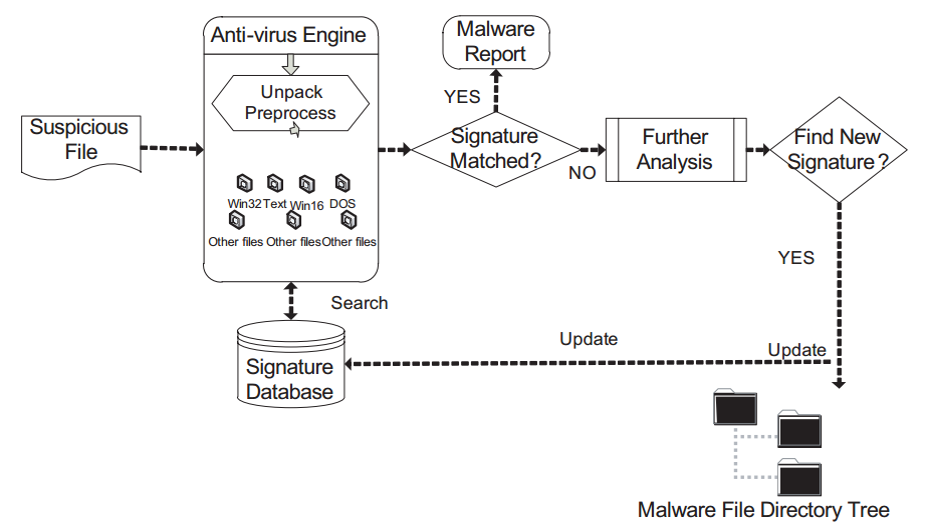
\includegraphics[width=4.5in]{img/intro/signatureFlow.png}
\caption{特征码匹配流程}
\label{fig:intro:signatureFlow}
\end{figure}

\subsection{静态分析与检测技术}
\subsection{动态分析与检测技术}

\makeatletter
\addtocontents{lof}{\vspace{-10pt}}
\addtocontents{lot}{\vspace{-10pt}}
\makeatother

\iffalse
\bibliography{../bib/thesis.bib}
\fi

\chapter{基于图的恶意软件静态分析方法研究}
\section{研究背景}

\section{基于图的恶意软件静态分析}
本方法的体系框架如图\ref{fig:chap1:Architecture}所示,由几个阶段构成。首先,反编译原始PE文件得到标准的汇编代码,经过预处理后抽象出控制流图(Control flow graph, CFG)。控制流图是用在编译器中的一个抽象数据结构,它是一个有向图,是过程或程序的抽象表现。在图中的每个节点代表一个基本块;每条有向边被用于代表在控制流中的跳跃,跳跃目标以一个块开始,以另一个块结束。其次,用调用的API或函数标记图中的每一条边,得到FA-CFG图;下一步,根据FA-CFG图建立特征向量,运用数据挖掘分类算法做出决策,判断该PE文件是否为恶意软件。

\begin{figure}[!ht]
\centering
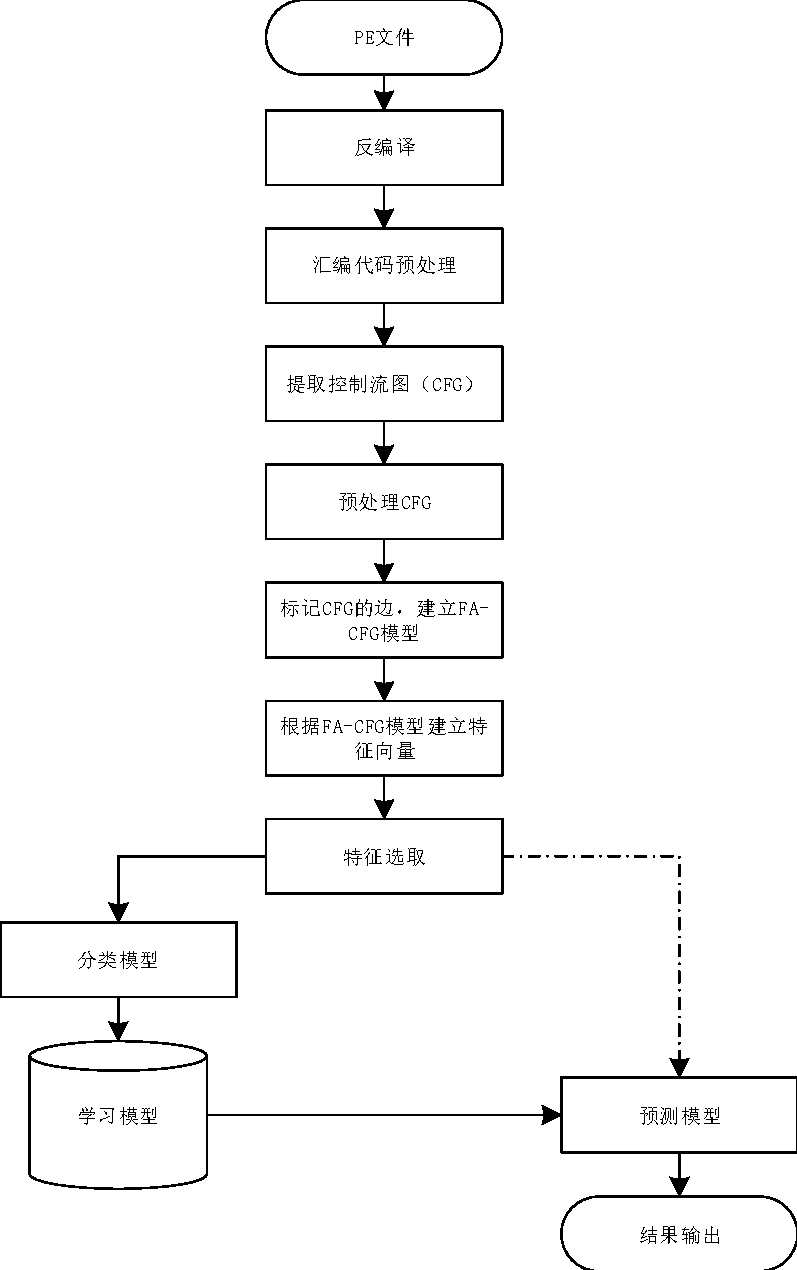
\includegraphics[width=4.5in]{img/chap1/Architecture.pdf}
\caption{体系框架图}
\label{fig:chap1:Architecture}
\end{figure}

如图\ref{fig:chap1:Architecture}所示,该方法由以下四个主要部分构成:PE文件反编译,FA-CFG图生成,特征提取、分类学习算法。第一步,通过反编译,得到输入PE文件的汇编代码;第二步,对得到的汇编代码进行预处理,移除一些不需要的指令代码,根据剩下的指令代码生成CFG图。根据API类库以及统计得到的调用函数的信息生成FA-CFG图。图中的一些边被对应的API或者调用函数的信息所标记。第三步,根据FA-CFG图提取特征,并采取主成分分析法(PCA)进行降维从而得到合理的特征向量。第四步,运用数据挖掘算法进行训练,形成学习模型。决策模块根据此模型判别一个输入PE文件是否为恶意。
\subsection{PE文件反编译及构建FA-CFG图}
静态分析方法中最主要的步骤是逆向工程。在静态分析中,通过检测代码来抓取恶意软件的行为。在不执行可疑软件的基础上使用逆向工程软件或反编译器来进行分析。逆向工程是编译的反过程,是从程序中以源代码的形式获得高层次的工程性描述或者说明的过程。它可以被用来对程序的执行计划、程序结构、算法进行仔细分析。在逆向工程的过程中,底层机器代码被反编译为汇编代码,进而汇编代码被反汇编成高级语言。通过逆向工程的分析可以得到程序的函数长度、可打印字符串、基本块、指令集、控制流图、调用关系图等信息。
在控制流图(CFG)中,每个节点代表一个基本块;每条有向边被用于代表在控制流中的跳跃,跳跃目标以一个块开始,以另一个块结束。在传统的控制流图中,每条边仅标识每次跳跃的开始与结束,没有反应跳跃的详细信息,包括调用的函数或API的信息等,因此,我们将函数调用和API调用产生的跳跃边用调用的详细进行标记,即可得到FA-CFG图。其中,函数调用所产生的边用所对应的函数的长度频率值标记,API调用所产生的边用对应API的ID标记。
\subsection{函数长度频率}
函数长度频率指函数代码长度在不同长度区间内的数量。将函数长度规模划分为几个不同的间隔,每个间隔称为一个容器。为每一个例子计算所有函数的长度在不同容器中的数量。由于函数长度的数量级差异,我们以指数增长的方式增加容器涵盖的范围。统计函数长度在1到$e$字节的数量,$e$字节到$e^{2}$字节的数量,以此类推。


\makeatletter
\addtocontents{lof}{\vspace{-10pt}}
\addtocontents{lot}{\vspace{-10pt}}
\makeatother

\iffalse
\bibliography{../bib/thesis.bib}
\fi

\chapter{基于标签传播的恶意软件检测算法研究}
恶意软件编程技术的快速发展已经给计算机和网络安全提出了巨大的挑战。因此,反病毒企业与市场急需发展新的有效的方法和框架来保护用户以应对更新的病毒威胁。现有的病毒软件检测技术主要将文件样本作为单一的个体,分析提取文件样本的特征,例如API调用序列、指令序列和二进制字符串等,再运用数据挖掘算法,如朴素贝叶斯、支持向量机等进行病毒检测。文件样本之间的关联关系隐含了大量有价值的信息,忽略他们的关联关系使得分析和检测恶意软件具有一定的局限性。本章从文件样本间关系的角度出发,研究文件样本之间的关联关系和关系类型,提出了基于标签传播的恶意软件检测模型,通过实验验证了标签传播算法在文件关系图上对检测恶意软件的准确性和有效性。
\section{相关研究}


\section{文件关联图的构建}
\subsection{文件关联图类型}
文件关联图根据关联类型以及参与者的不同而不同,
\begin{asparaenum}
\item 文件—文件(File-File)。在文件—文件关联图中,文件与文件之间直接建立关联,若两个文件有共存关系或者有一定的相似度,则就在图中用一条边连接这两个文件对应的节点。
\item 文件—设备(File-Machine)。在文件—设备关联图中,与文件直接相连的是文件所存在的设备(个人电脑、计算机、手机、智能终端等)。通过设备作为过渡点,文件与文件之间建立间接的联系。
\item 文件—聚类(File-Cluster)。在文件—聚类关联图中,通过某种相似度评价算法(例如局部敏感哈希,LSH)将文件在不同维度上进行聚类操作,因此可能会导致同一个文件在不同的维度上会被分到多个聚类中。根据文件与聚类之间的关系,建立文件—聚类关联图。通过聚类作为过渡,文件与文件之间建立间接的联系。
\item 文件—特征(File-Feature)。在文件—特征关联图中,提取文件的特征属性并根据文件属性的紧密程度建立文件与特征间的关系。例如,对于每个Android程序,在AndroidManifest.xml需要声明改程序所需的系统操作权限,将每一种权限作为一个特征即可建立文件与特征之间的关系,即某一权限在程序中被声明则就建立程序与这个特征的联系。
\end{asparaenum}

后三种图均可为二部图,即图中的节点可以分为两部分,一部分为文件,另一部分为另一种实体(即设备、聚类或特征),分属两个部分内的节点互相连接,同一部分内部的节点没有直接连接。本章采用文件—文件关系类型构建文件关联图。
\subsection{图的构建策略}
\label{sec:graphStrategy}
在基于图的半监督学习中,一个良好的图构建方法至关重要。在长期的理论和实践中发现,图的构建方法对最终算法的性能有着重要的影响,甚至在某些情况下构建图的方法比算法更加重要。Maier\cite{maier2008influence}等人研究发现,对于相同的数据以及相同的聚类算法,不同的图构建方法可能会得到不同的结果。Zhu\cite{zhu2005semi}认为能够体现半监督学习假设(半监督平滑性假设、聚类假设和流行假设等)的图才是一个好图。下文列举几种图的构造方法:
\begin{asparaenum}
\item 全连图(Fully connected graphs)。将任意两个节点$v_{i}$和$v_{j}$用一条边连接起来所形成的图称为全连图。相似度较高的两个节点之间的边有较高的权值。全连图的优点是构造方法简单,每条边都被赋予一个权重值(一个可导的权重函数),通过求导的方法即可快速的求解。但是全连图也有明显的缺点,由于任意两个点之间都有边相连,导致了求解过程中庞大的运算量。
\item $k$近邻图($k$-nearest-neighborhood graphs)。若节点$v_{j}$是节点$v_{i}$最近的$k$个近邻之一,则用一条边将这两个节点相连。$k$是控制整个图密度的超参数。$k$近邻图具有良好的自适应性,当样本空间的密度较大时,$k$近邻图的半径就比较小;反之,当密度较小时,图的半径就比较大。在近邻图中,节点$v_{i}$是节点$v_{j}$的$k$近邻并不代表节点$v_{j}$也是节点$v_{i}$的$k$近邻。在构建$k$近邻图时,只要其中一个节点是另一个节点的$k$近邻,则就用一条边连接两个节点,因此在$k$近邻图中每个节点的度(即关联的边数)可能大于$k$。
\item $\epsilon$近邻图($\epsilon$-neighbors graphs)。若节点$v_{i}$和$v_{j}$的距离$d(v_{i},v_{j})\leqslant \epsilon$,则用一条边来连接两个节点。超参数$\epsilon$控制了近邻的半径大小,影响了构造图的连通性。
\item $exp$权重图($exp$-weighted graphs)。上述三种图构造方法主要集中于图的结构构建,没有详细规范图中边权重的计算方法。而$exp$权重图提出了不同的权重计算方法。根据公式$w_{ij}=exp(-d(v_{i},v_{j})^{2}/{\sigma}^{2})$计算连接两个节点的边的权重。超参数$\sigma$影响了权值的衰变。拓展开来,可以为特征的每一维都指定一个超参数$\sigma$。$exp$权重图可以和上述三种构造方法配合使用完成图的构造过程。
\end{asparaenum}

\subsection{构建文件关联图}
\label{sec:fileGraph}
在本章中,我们通过文件样本之间的共存度作为衡量文件样本相似度的标准,以此构建文件样本关联图。定义文件关联图为$G=(V,E,W)$,其中$V$为代表文件样本的节点的集合,$E$为文件样本节点间关系的集合,$e(v_{i},v{j})\in E$,$v_{i}, v_{j}\in V$,表示存在一条边连接节点$v_{i}$和$v_{j}$,$W$为每一条边的权重,即边连接的两个节点的相似度。设$C_{i}$为节点$v_{i}$对应的文件$f_{i}$存在的终端集合。这里我们运用Jaccard相似度来衡量两个文件的共存度,公式如下:
\begin{equation}
sim(f_{i},f_{j})=\frac{\left | C_{i}\cap C_{j} \right |}{\left | C_{i}\cup C_{j} \right |},
\end{equation}
其中,$\left | C \right |$是集合$C$的大小,即文件存在的终端总数。可以看出,共存度的取值是一个介于0和1之间的数。``0''表示两个文件之间没有共存关系,即从未同时存储在同一台终端上; 反之,``1''则表示两个文件之间存在完全的共存关系,可能两个文件存在某种依赖关系。

在实际应用中,文件样本及其存储信息是从实际的用户客户端中采集而来,采集所有的文件样本以及所有的共存信息是不现实、不可行的,因此我们只采集可疑的文件样本以及与已标记文件的共存关系,这就导致了未标记文件样本之间共存关系的丢失。我们使用未标记文件与已标记文件的共存关系来估算未标记文件间的相似度。令$M_{i}$为未标记文件$f_{i}$共存的已标记样本的集合,则未标记文件$f_{i}$和$f_{j}$的相似度为:
\begin{equation}
sim(f_{i},f_{j})=\sum_{m\in M_{i}\cap M_{j}}sim(m,i)*sim(m,j).
\end{equation}

在\ref{sec:graphStrategy}小节,我们讨论了图的构建策略和常用的几种方法。在本章中,我们使用$k$近邻图的构建策略来构建文件关联关系图,若文件样本$f_{i}$是文件$f_{j}$的$k$近邻,则用一条边连接它们,且边的权重为两者的相似度。

为清晰的说明文件关联图构建过程,这里我们选取了一个文件关联的数据集作为例子,如表\ref{tb_dataSample}所示。第一列为文件的ID;第二列为文件的标记,``0''代表当前文件为未标记样本,``1''代表当前文件为良性文件,``-1''代表当前文件为恶意软件;第三列为当前文件样本与恶意软件样本的共存记录;第四列为当前样本与良性文件样本的共存记录;第五列为文件样本存在的终端总数。举例来说,ID为2的文件样本,它是一个存在于两个终端的未标记样本,与ID为4的恶意软件样本共存于一台终端中,与ID为3和ID为6的良性文件样本分别共存于两台终端中。根据所给示例数据,我们选择$k=3$(选择每个节点最近的3个近邻)构建文件关联图,如图\ref{fig:SampleGraph}所示。它是一个无向带权图,图中节点旁标注的数值代表了节点对应的文件样本的编号,同理,每条边上的数值为边的权重,即两节点的相似度。
\begin{table}[!ht]
\caption{文件关联数据库范例}
\label{tb_dataSample}
\centering
\begin{tabular}{ccccc}

\toprule
ID & 标签 & 与恶意软件的共存信息 & 与良性文件的共存信息 & 客户端数量\\
\midrule
1 & 0 & 7(1),8(1),10(1) & 6(1) & 2\\
2 & 0 & 4(1) & 3(2),6(2) & 2\\
3 & 1 & 4(1),8(1) & 5(2),6(3) & 4\\
4 & -1 & 8(1),10(1) & 3(1),6(1) & 2\\
5 & 1 & 8(1) & 3(2),6(1) & 2\\
6 & 1 & 4(1),8(1) & 3(3),5(1) & 4\\
7 & -1 & 10(1) & ------ & 1\\
8 & -1 & 4(1),10(1) & 3(1),5(1),6(1) & 3\\
9 & 0 & ------ & 3(1),5(1),6(1) & 1\\
10 & -1 & 4(1),7(1),8(1) & ------ & 2\\
\bottomrule
\end{tabular}
\end{table}

\begin{figure}[!t]
\centering
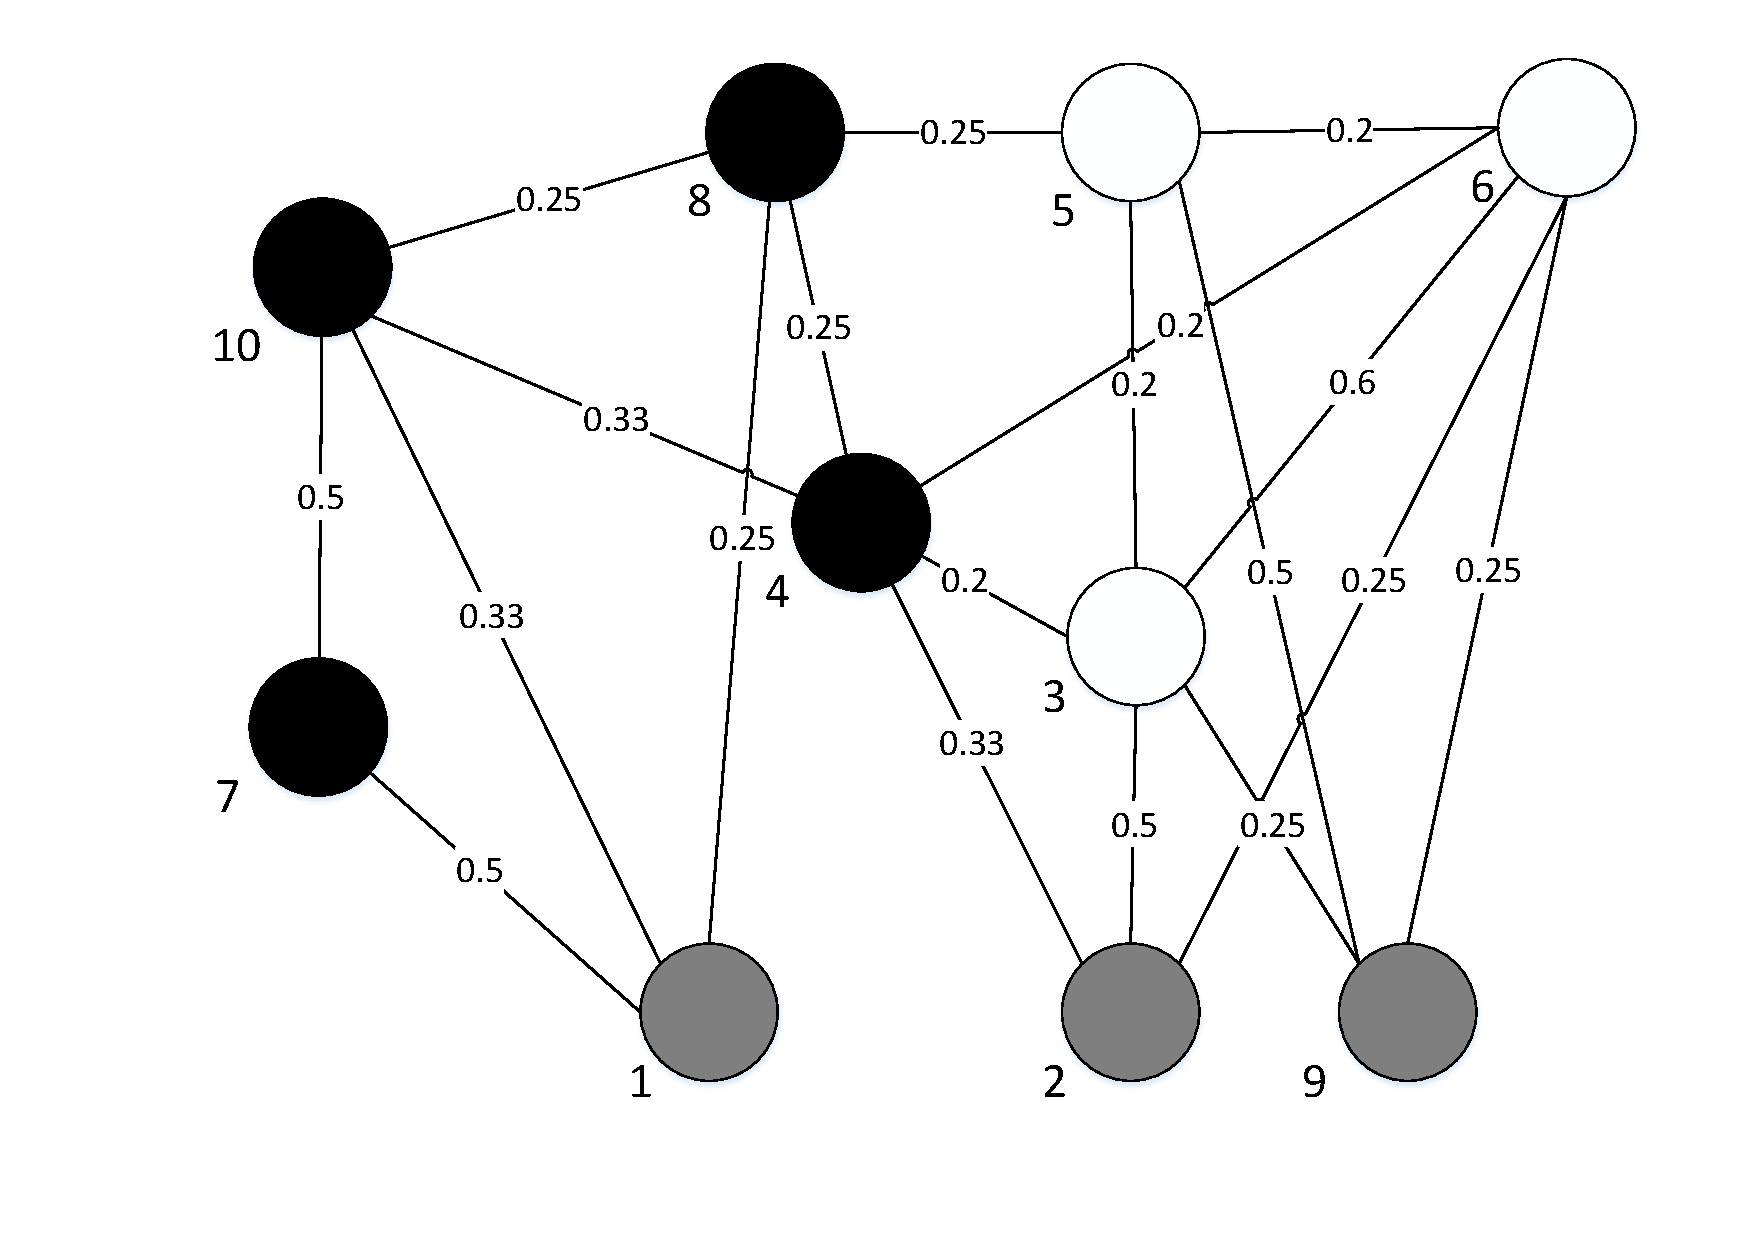
\includegraphics[width=4.5in]{img/chap2/SampleGraph.pdf}
\caption{基于表\ref{tb_dataSample}的文件关联图示例}
\label{fig:SampleGraph}
\end{figure}

\section{标签传播算法}
\label{sec:lp}
数据挖掘算法中,标签数据对于监督学习算法是必需的。然而在很多模式分类的实际应用中,由于样本的标记工作需要昂贵的人力、财力和时间成本,获取大量的标记样本是不实际的。因此,在通常情况下我们面对的是少量的标记样本和大量的未标记样本。如何将未标记样本和标记样本结合起来共同训练模型是近几年研究的热点。

2002年,Zhu等人提出了标签传播算法(LPA,Label Propagation Algorithm)\cite{zhu2002learning},它是一种基于图的半监督学习方法,其基本思想为将已标记节点的标签信息传递给未标记节点以预测未标记节点的标签,高相似度的数据节点倾向于属于同一类别。根据样本间的关系构建关系完全图模型,其中包括已标记节点和未标记节点,节点与节点间的关系则用边来表示,节点间的相似度则表示为边的权重。在标签传递的过程中,已标记节点的标签信息根据节点间的相似度进行传递给邻接节点乃至整个图直至所有的未标记节点达到稳定的标签状态。

标签算法具体如下:设$D_{L}=\left \{ (x_{1},y_{1})...(x_{l},y_{l}) \right \}$为已标记数据,其中$\left \{ y_{1}...y_{l} \right \}$是类别标签。假设类别总数$\left | C \right | $已知,且所有的类别在已标记数据中均存在。令$D_{U}=\left \{ (x_{l+1},y_{l+1})...(x_{l+u},y_{l+u}) \right \}$为未标记数据,$\left \{ y_{l+1}...y_{l+u} \right \}$是不可观测的,通常$l\ll u$(即已标记数据占比很低,未标记数据的数量远大于已标记数据的数量)。该算法的最终目的即为,根据数据集$X$和已知数据标签$\left \{ y_{1}...y_{l} \right \}$来估计$\left \{ y_{l+1}...y_{l+u} \right \}$的取值。

根据数据集中的数据(包括已标记数据和未标记数据)创建一个完全连通图,其中图中每一个节点表示了数据集中的一条数据。节点$i$和$j$之间边的权重用节点间的相似度表示,如下公式:
\begin{equation}
\label{eq:lp_distance}
w_{ij}=\exp\left ( -\frac{d_{ij}^{2}}{{\sigma}^{2}} \right )=\exp\left ( -\frac{{\sum}_{d=1}^{D} {(x_{i}^{d}-x_{j}{d})}^2}{{\sigma}^{2}} \right ),
\end{equation}
其中,$d_{ij}$为两点之间的距离。这里使用欧式距离计算,也可以使用其他的距离计算方法。

定义一个$(l+U)\times C$标签矩阵$Y$,令$Y_{ij}$为节点$x_{i}$被标记为类别$y_{i}$的概率。换言之,矩阵$Y$表示了图中每一个节点的标签概率分布。为衡量节点将标签信息传递给邻接节点的能力,定义概率传递矩阵$T$,
\begin{equation}
\label{eq:lp_transition}
T_{ij}=P(j\rightarrow i)=\frac{w_{ij}}{\sum_{k=1}^{l+u}w_{ij}},
\end{equation}
其中,$T_{ij}$表示从节点$j$跳转到节点$i$的概率,即节点$j$传递标签信息给节点$i$的概率。该算法描述如下:
\begin{asparaenum}
\item 根据公式\ref{eq:lp_distance}计算数据间的相似度以初始化权重矩阵$W$, 并根据矩阵$W$和公式\ref{eq:lp_transition}计算节点$j$到$i$的传播概率,得到标签传递矩阵$T$。
\item 根据已标记数据的标签信息初始化标签矩阵$Y$;若节点$y_{i}$属于类别$C_{j}$,则$Y_{ij}=1$,否则$Y_{ij}$为0。
\item 每个节点将其标签信息传递给邻接节点,其中矩阵$\overline{T}$由矩阵$T$按行归一化得到。
\item 将已标记数据的标签重置为初始值,保证原始的标签信息能够正确传播。重复上一步骤,直至收敛。
\item 根据$y_{i}={\arg \max}_{j}Y_{ij}$,为未标记节点分配标签。
\end{asparaenum}

\begin{algorithm}
\caption{标签传播算法(LPA)}
\label{alg:lp}
\begin{algorithmic}[1]
\Input 未标记数据$D_{U}=(x_{l+1},y_{l+1})...(x_{l+u},y_{l+u})$, 标记数据$D_{L}=(x_{1},y_{1})...(x_{l},y_{l})$及类别集$C$
\Output 未标记数据的类别
\State $initial(D_{U}, D_{L})$ \Comment{初始化相似度矩阵$W$和标签传递矩阵$T$}
\For{$i=0; i<l+u; i++$} \Comment{初始化标签矩阵$Y$}
\For{$j=0; j<\left | C \right | ; j++$}
\State $Y_{ij} = p(y_{i},C_{j})$
\EndFor
\EndFor
\Repeat
\State $Y\leftarrow \overline{T}Y$ \Comment{传播标签信息}
\label{code:lp:propagate}
\State $clamp(D_{L})$ \Comment{限定已标记数据}
\label{code:lp:clamp}
\Until {$Y$ converges}
\State $assignLabel(D_{U})$
\end{algorithmic}
\end{algorithm}

算法\ref{alg:lp}描述了标签传播算法(LPA)的具体步骤。根据已标记数据和未标记数据的排列顺序,划分行规一化矩阵$\overline{T}$为如下4个子矩阵:
\begin{equation}
\overline{T}=\begin{bmatrix}
\overline{T}_{ll} & \overline{T}_{lu} \\ 
\overline{T}_{ul} & \overline{T}_{uu}
\end{bmatrix}
\end{equation}
在算法迭代过程中,由于已标记数据的标签信息始终被限定为原始信息,因此标签矩阵$Y$中前$l$行即子矩阵$Y_{L}$保持不变,算法改变的是未标记数据的部分即子矩阵$Y_{U}$。故算法第\ref{code:lp:propagate}行可改写为
\begin{equation}
Y_{U} \leftarrow \overline{T}_{uu}Y_{U}+\overline{T}_{ul}Y_{L}
\end{equation}
经过有限次迭代后,可以证明该算法收敛至唯一值$Y_{U}=(I-\overline{T}_{uu})^{-1}\overline{T}_{ul}Y_{L}$。

标签传播算法(LPA)只需利用少量的标记数据作为学习导向,利用未标记数据的内部结构和分布规律,即可传播已标记数据的标签信息以及预测未标记数据的标签。该算法操作简单、运算量小,适合大规模数据信息的挖掘和处理。

\section{算法描述}
结合\ref{sec:fileGraph}节构建的文件关联图和\ref{sec:lp}节描述的标签传播算法,我们提出基于标签传播的恶意软件检测算法。在原始的标签传播算法中,根据原始数据点构造了一个完全连通图,在此图的基础上传播节点的标签信息以完成未标记节点的标签学习。本章提出的算法是基于文件样本之间的关联信息的,因此我们单独提出了文件关联关系图的构造策略和算法,以此改进原始标签传播算法中关系图的构造方法。算法\ref{alg:md}阐述了该方法的具体步骤。

\begin{algorithm}
\caption{基于标签传播的恶意软件检测算法}
\label{alg:md}
\begin{algorithmic}[1]
\Input 原始文件列表数据$FileList$
\Output 文件样本的标签
\For{each $f_{i}$ in $FileList$}\Comment{计算每个文件与已知关联文件之间的相似度}
\State $similaityASS(f_{i})$
\EndFor
\For{each $f_{i}$ in $FileList$}\Comment{计算未标记文件样本之间的相似度}
\For{each $f_{j}$ in $FileList$}
\If{$f_{i}$ is unlabled and $f_{j}$ is unlabled}
\State $similaityUnLabel(f_{i},f_{j})$
\EndIf
\EndFor
\EndFor
\State $createGraph(V,E,W,k)$\Comment{构造$k$近邻图}
\State 根据算法\ref{alg:lp}所述的算法进行标签传播
\State 根据标签矩阵标记未标记文件样本的标签
\end{algorithmic}
\end{algorithm}


\section{实验验证}
在本章中,我们提出了一种基于标签传播的恶意软件检测方法,本节将通过两组实验分别来验证算法的可行性和有效性。在第一组实验中,将验证$k$近邻图对于算法准确率的提升并通过实验选择最佳的$k$值;第二组实验将对比本算法与其他基准算法,以验证本算法对恶意软件检测的有效性。

本章中实验的实验环境基于一台普通PC,设备配置为Intel Core i7 2.7G Hz Duo CPU、8GB RAM和500GB硬盘存储,搭建的实验平台为Windows 8操作系统以及JAVA 1.7编程环境。实验过程中使用的性能评价指标如下:
\begin{itemize}
\item \textbf{True Positive(TP)}: 被正确标记为恶意的样本数量。
\item \textbf{True Negative(TN)}: 被正确标记为良性的样本数量。
\item \textbf{False Positive(FP)}: 被错误标记为恶意的样本数量。
\item \textbf{False Negative(FN)}: 被错误标记为良性的样本数量。
\item \textbf{TP Rate(TPR)}: $\frac {TP} {TP+FN}$
\item \textbf{FP Rate(FPR)}: $\frac {FP} {TN+FP}$
\item \textbf{Accuracy(ACC)}: $\frac {TP+TN} {TP+TN+FP+FN}$
\end{itemize}

\subsection{实验数据}
\label{sec:DataDes}
本节介绍实验中所用数据集的相关信息。该数据集由某安全软件企业从真实客户中收集而来,包含69,165个文件样本(其中包括3,095个恶意软件、22,583个良性文件以及43,487个未知文件)以及这些样本之间的关联关系\cite{ye2011combining}。图\ref{fig_Database}为文件关联数据库的结构,包括8个字段:文件ID,文件标签(``1'' 表示当前文件为良性文件, ``-1''表示当前文件为恶意软件,  ``0''代表当前文件为未知文件),文件名,与当前文件共存的恶意软件数量,与当前文件共存的恶意软件ID列表,与当前文件共存的良性文件数量,与当前文件共存的良性文件ID列表,文件存储的客户端数量。

\begin{figure}[!ht]
\centering
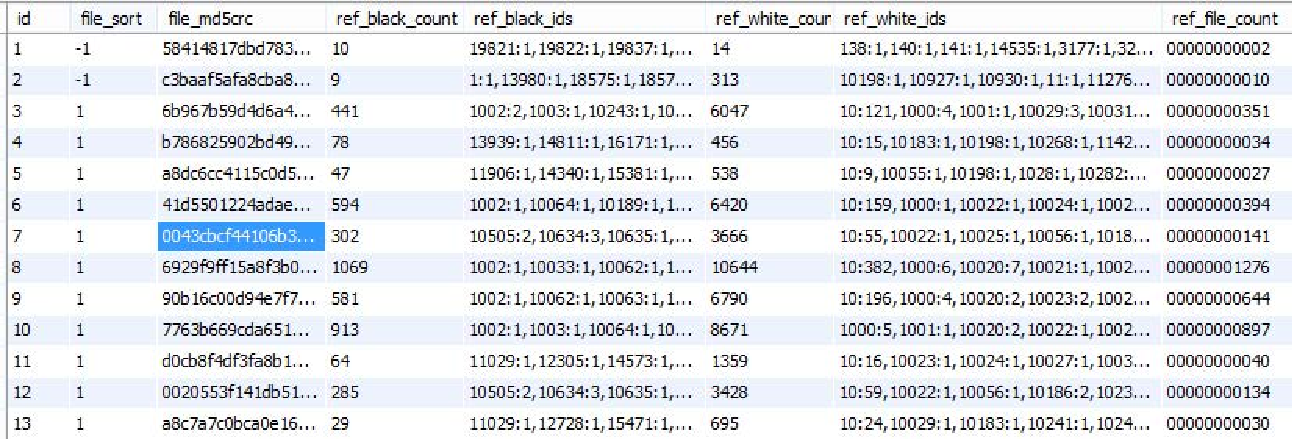
\includegraphics[width=3.5in]{img/chap2/Database.pdf}
\caption{文件关联关系数据库}
\label{fig_Database}
\end{figure}

通过对数据集的分析发现,良性文件的数量远比恶意软件大的多,因此导致了数据分布的不均衡,当然,不仅仅是文件样本数量分布的不均衡,文件之间的关联关系也存在着不均衡分布。图\ref{fig_MalRef}和图\ref{fig_MalRefWht}分别汇总了恶意软件与恶意软件之间的共存关系以及恶意软件与良性文件之间的共存关系。

\begin{figure}[!ht]
\centering
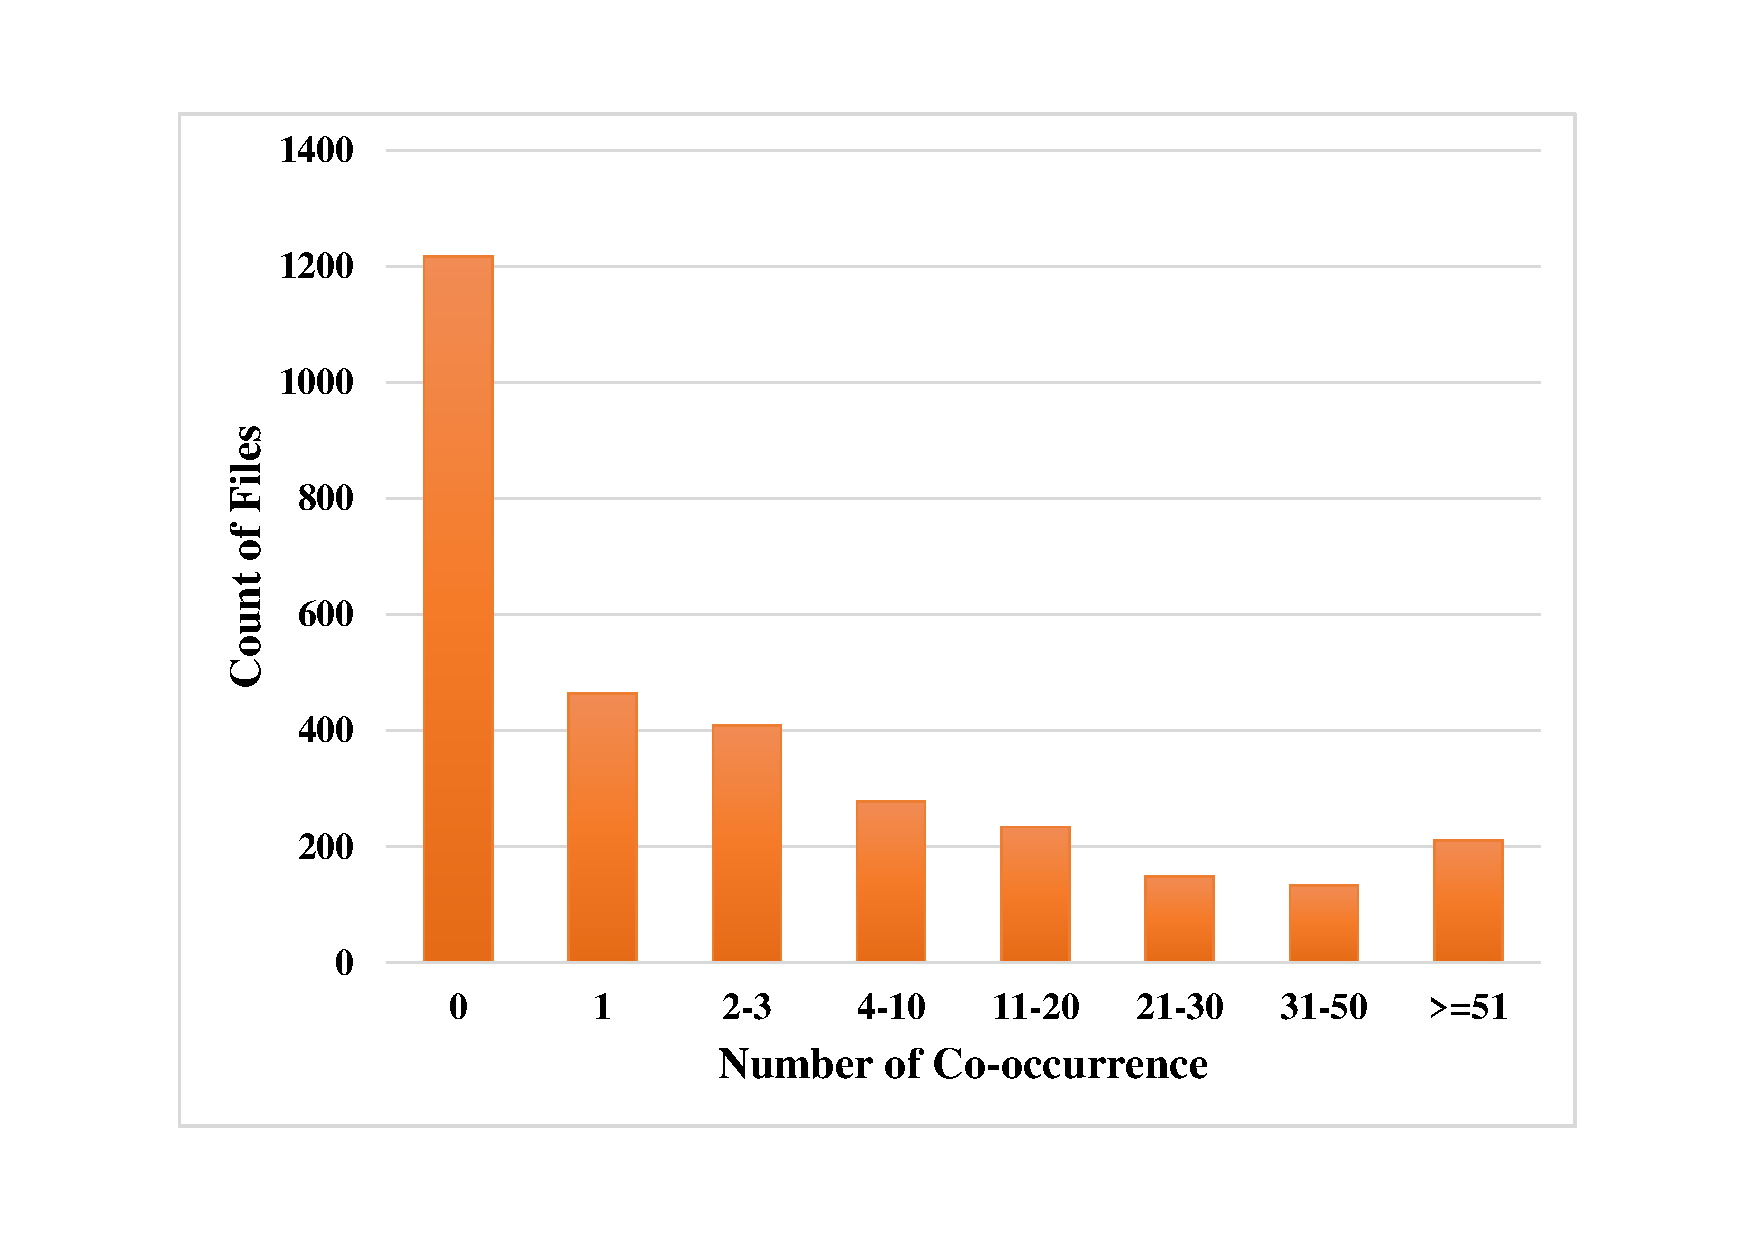
\includegraphics[width=3.5in]{img/chap2/MalRefCount.pdf}
\caption{恶意软件与恶意软件之间的共存关系}
\label{fig_MalRef}
\end{figure}

\begin{figure}[!ht]
\centering
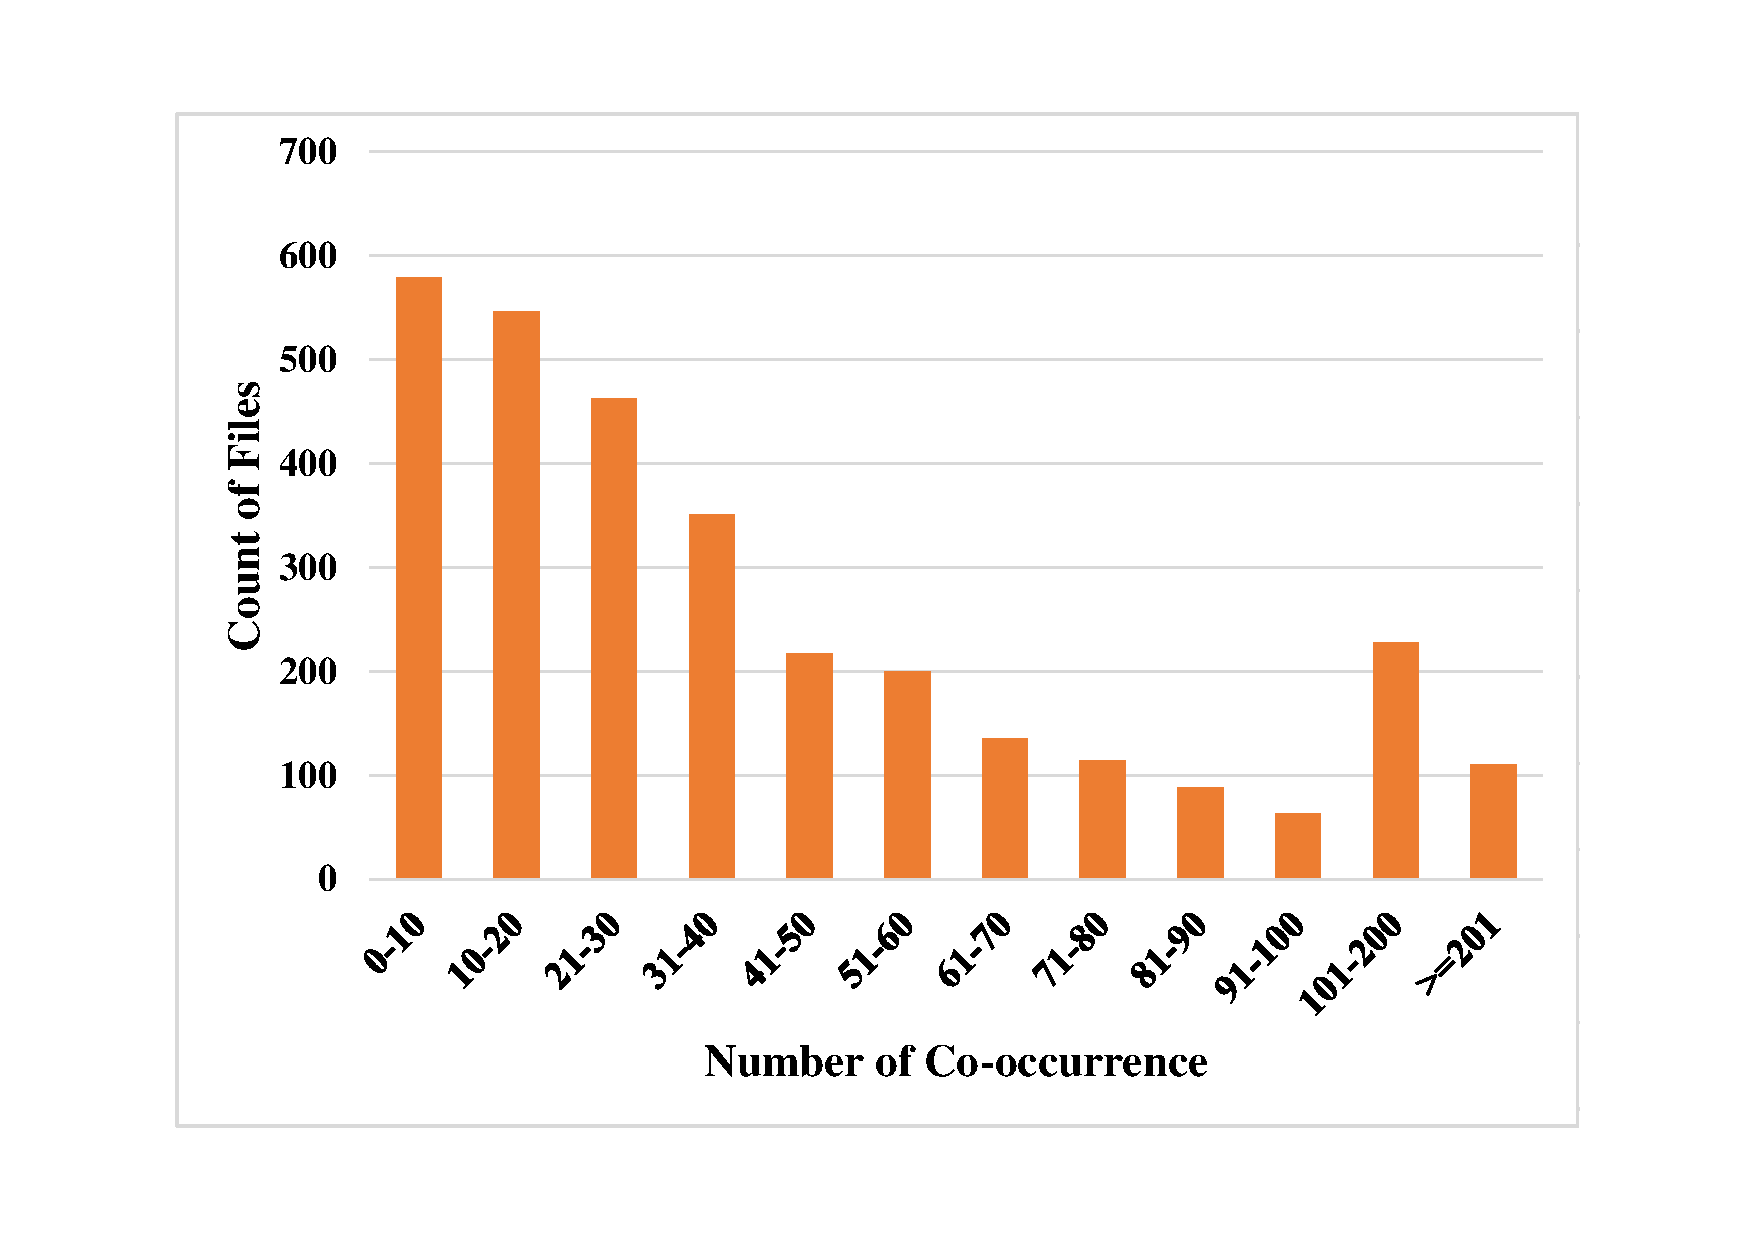
\includegraphics[width=3.5in]{img/chap2/MalRefCountWht.pdf}
\caption{恶意软件与良性文件之间的共存关系}
\label{fig_MalRefWht}
\end{figure}
在本章的实验中,我们从已标记文件样本中随机抽取了3,986个文件(其中包括289个恶意软件,3,697个良性文件)作为测试集,剩余样本作为训练集。

\subsection{$k$NN图构建性能对比分析}
在构建文件关联图时,我们使用了$k$近邻策略过滤数据噪声并选择每个文件样本最相似的邻居样本。本节选择与全连图、$\epsilon$近邻图进行实验对比,验证$k$近邻图的有效性。这里分别选择$\epsilon=0.01$、$\epsilon=0.02$、$\epsilon=0.05$、$\epsilon=0.07$和$\epsilon=0.1$以及$k=10$、$k=30$、$k=50$、$k=70$和$k=100$作为构图参数。通过表\ref{tb_ResKNN}和图\ref{fig_ReskNN}可以看出,运用$k$近邻策略能够明显的提升算法的有效性和准确率。当$k=50$时,对比全连图策略,$k$近邻策略在TP(True Positive)和TN(True Negative)测度上分别能够获得41\%和6.9\%的提高,准确率则可以提升7.96\%。

\begin{table}[!ht]
\renewcommand{\arraystretch}{1.5}
\caption{$k$近邻图性能对比}
\label{tb_ResKNN}
\centering
\begin{tabular}{cccccccc}

\toprule
 & TP & FP & TN & FN & TPR & FPR & ACC\\
\midrule
全连图 & 110 & 301 & 3,396 & 179 & 0.38 & 0.08 & 0.8796 \\
$k=10$ & 109 & 224 & 3,473 & 180 & 0.38 & 0.06 & 0.8986 \\
$k=30$ & 113 & 179 & 3,518 & 176 & 0.39 & 0.05 & 0.9109 \\
$k=50$ & 155 & 67 & 3,630 & 134 & \textbf{0.54} & 0.02 & \textbf{0.9496}\\
$k=70$ & 126 & 139 & 3,558 & 163 & 0.44 & 0.04 & 0.9242 \\
$k=100$ & 122 & 199 & 3,498 & 167 & 0.42 & 0.05 & 0.9082 \\
\bottomrule
\end{tabular}
\end{table}

\begin{figure}[!ht]
\centering
\subfigure[TP VS FN]{
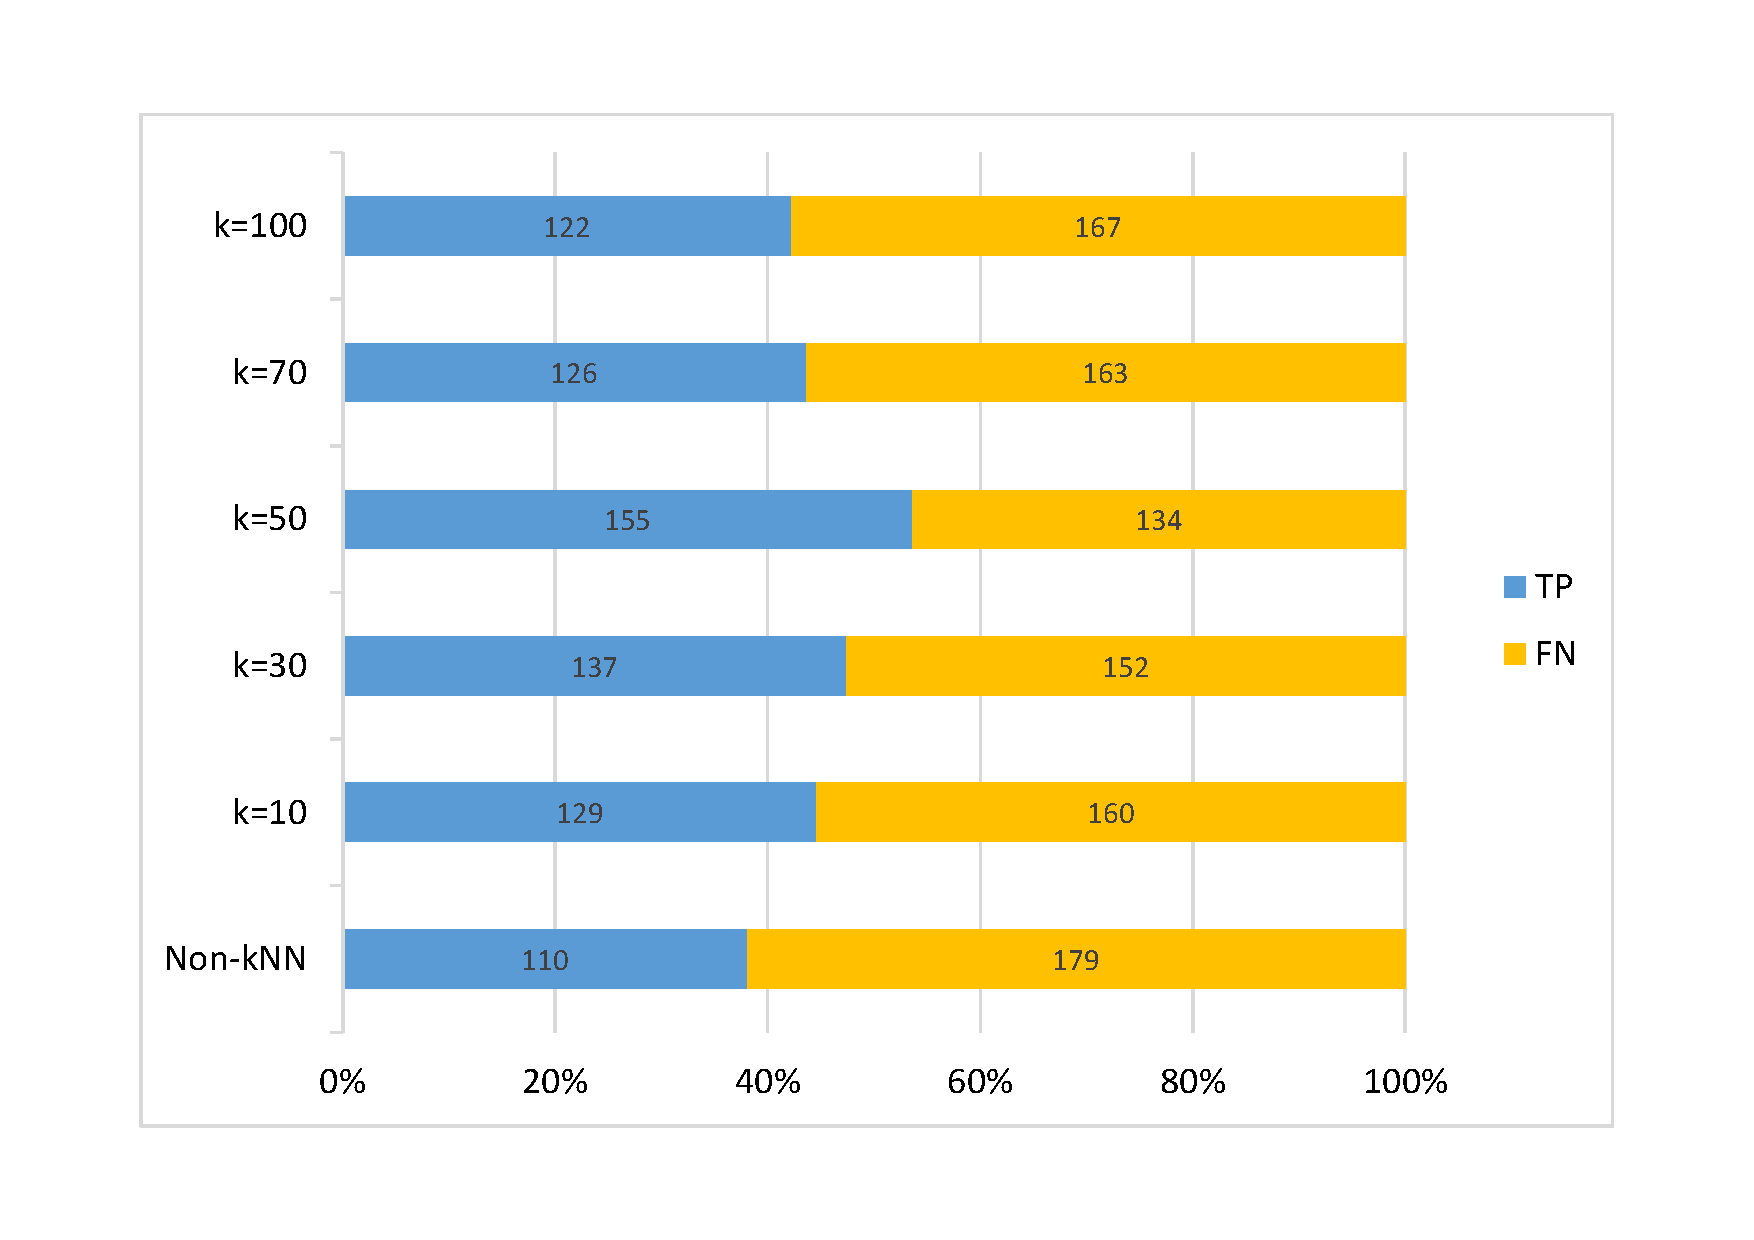
\includegraphics[width=4in]{img/chap2/ResultkNN_TP.pdf}
}
\subfigure[TN VS FP]{
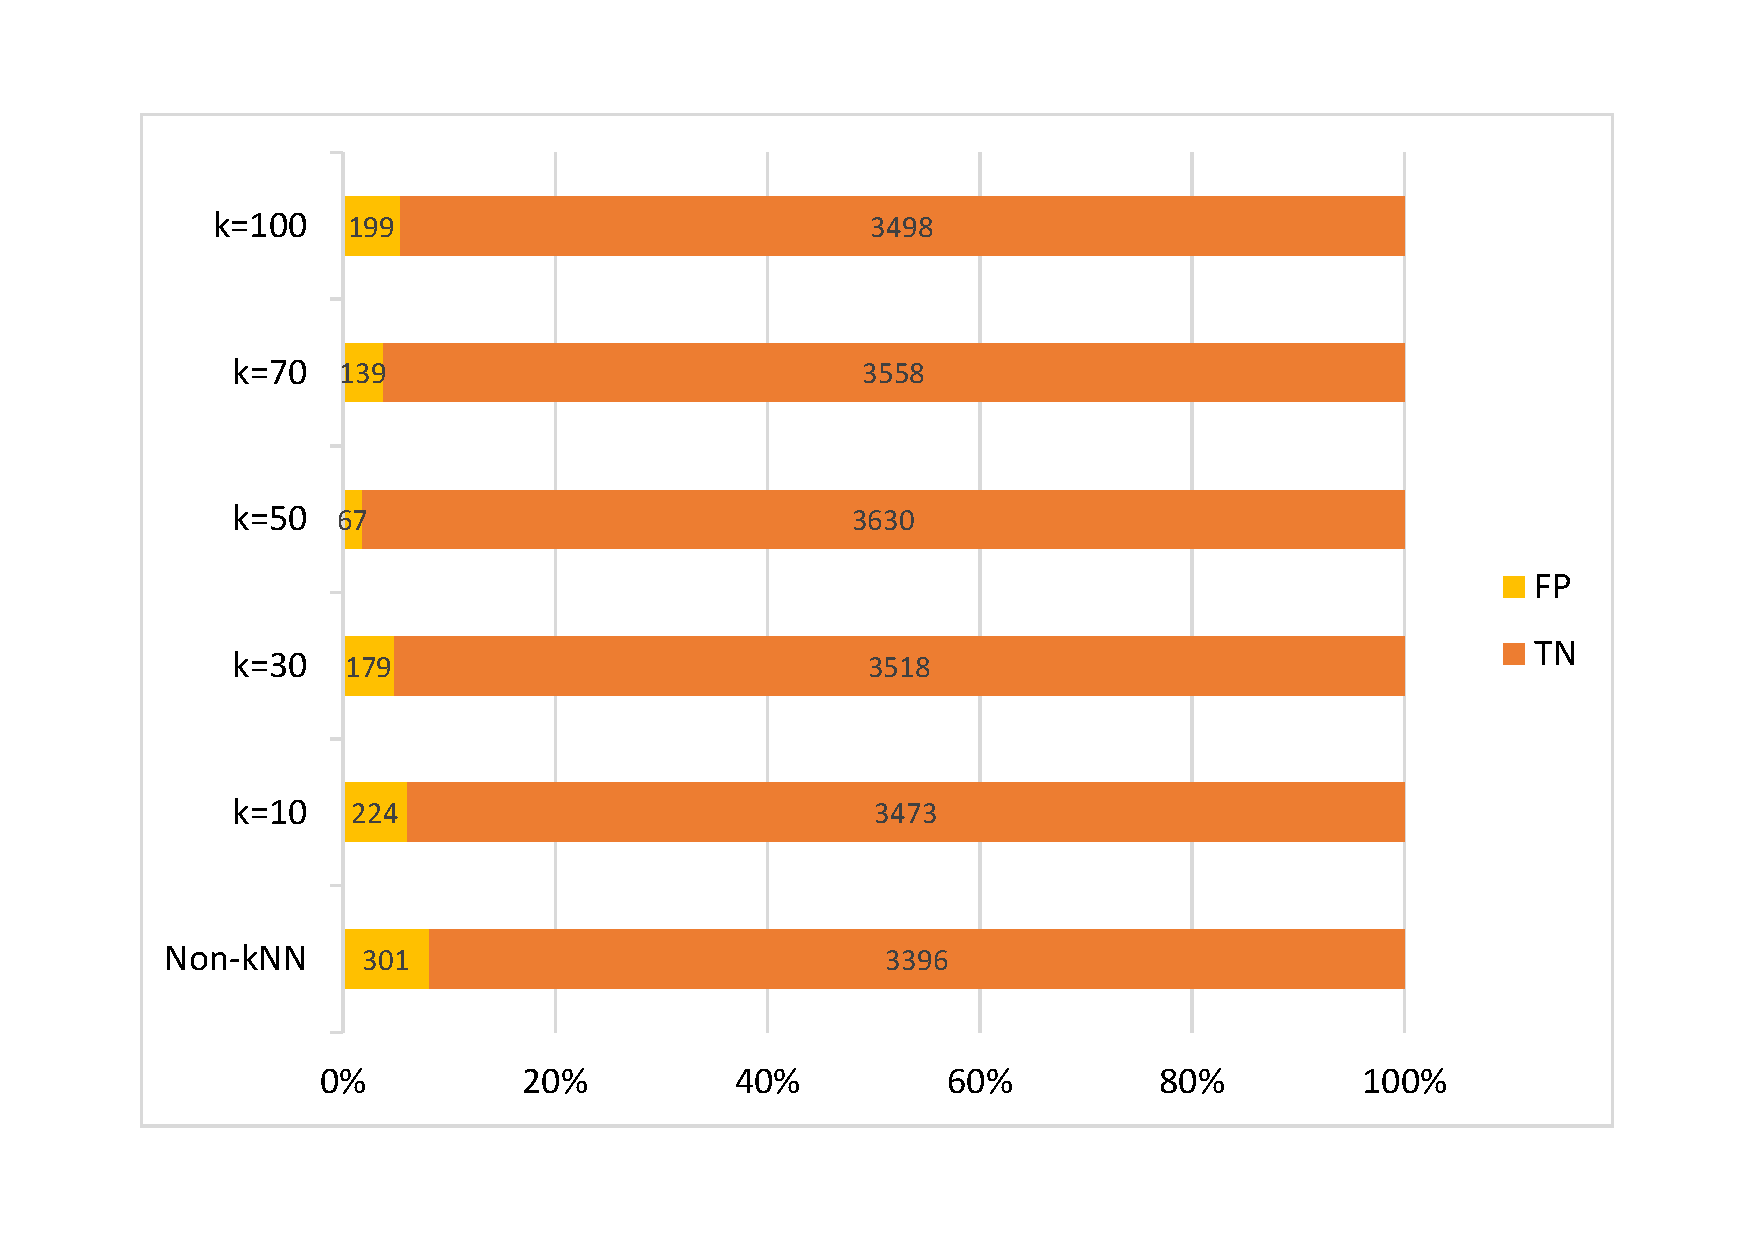
\includegraphics[width=4in]{img/chap2/ResultkNN_TN.pdf}
}
\caption{$k$近邻图性能对比}
\label{fig_ReskNN}
\end{figure}

同时,对比表\ref{tb_ResGraph}和表\ref{tb_ResKNN}的结果,可以看出$k$近邻策略的在每个测度上普遍都优于$\epsilon$近邻图的测度。尤其当$k$取值为50时,算法的准确率明显的高于$\epsilon$近邻图的最优情况。以上实验也验证了$k$取值为50时本算法能够取得最优性能。

\begin{table}[!ht]
\renewcommand{\arraystretch}{1.5}
\caption{三种构图策略对比}
\label{tb_ResGraph}
\centering
\begin{tabular}{cccccccc}
\toprule
 & TP & FP & TN & FN & TPR & FPR & ACC\\
\midrule
全连图 & 110 & 301 & 3,396 & 179 & 0.38 & 0.08 & 0.8796 \\
$\epsilon=0.01$ & 106 & 246 & 3,451 & 183 & 0.37 & 0.8924 \\
$\epsilon=0.02$ & 115 & 213 & 3,484 & 174 & 0.40 & 0.06 & 0.9029 \\
$\epsilon=0.05$ & 121 & 184 & 3,513 & 168 & 0.42 & 0.05 & 0.9117 \\
$\epsilon=0.07$ & 132 & 140 & 3,557 & 157 & 0.46 & 0.04 & 0.9255 \\
$\epsilon=0.1$ & 125 & 174 & 3,523 & 164 & 0.43 & 0.05 & 0.9152\\
$k=50$ & 155 & 67 & 3,630 & 134 & \textbf{0.54} & 0.02 & \textbf{0.9496}\\
\bottomrule
\end{tabular}
\end{table}


\subsection{算法性能分析}
本节将本章提出的恶意软件检测算法与现有的四个恶意软件检测算法进行比较,进一步验证算法的可行性和有效性。四个基准比较算法分别为:AESOP\cite{tamersoy2014guilt}、Malware Distributor Detector(MDD)\cite{venzhega2013graph}、支持向量机(Support Vector Machine, SVM)以及随机森林(Random Forest, RF)。其中,AESOP算法和Malware Distributor Detector算法同样是基于图的算法,因此可以根据文件的关联关系构造算法所需的关联关系图;而支持向量机算法和随机森林算法是基于特征属性的训练算法,因此我们定义每个文件样本的关联属性向量作为训练算法的特征向量:
\begin{equation}
R_{v_{i}}=\left \langle v_{1i},v_{2i},...,v_{ni}\right \rangle
\end{equation}
其中,
\begin{equation}
v_{ji}=\left\{\begin{matrix}
1 & (v_{j},v_{i}) \in E\\ 
0 & \text{其他}
\end{matrix}\right.
\end{equation}
根据上一组实验结果的分析,在构建文件关联关系图时,我们取$k$值为50。

\subsubsection{预测}
从表\ref{tb_ResComparisonWithBaseline}和图\ref{fig_ResComparisonWithBaseline}中可以看出,对比其他几种基准方法,本章提出的基于标签传播的恶意软件检测算法能够有效的发现数据集中的恶意文件样本,在大规模的现实数据中具有较好的表现。

\begin{table}[!ht]
\renewcommand{\arraystretch}{1.5}
\caption{在大规模现实数据上算法的性能对比}
\label{tb_ResComparisonWithBaseline}
\centering
\begin{tabular}{cccccccc}

\toprule
 & TP & FP & TN & FN & TPR & FPR & ACC\\
\midrule
Label Propagation & 155 & 67 & 3,630 & 134 & 0.54 & 0.02 & \textbf{0.9496}\\
AESOP & 198 & 3,385 & 312 & 91 & 0.69 & 0.92 & 0.1279 \\
MDD & 98 & 2,493 & 1,204 & 191 & 0.34 & 0.67 & 0.3266 \\
SVM & 81 & 461 & 3,236 & 208 & 0.28 & 0.12 & 0.8321\\
RF & 69 & 398 & 3,299 & 220 & 0.24 & 0.11 & 0.8449 \\
\bottomrule
\end{tabular}
\end{table}

\begin{figure}[!ht]
\centering
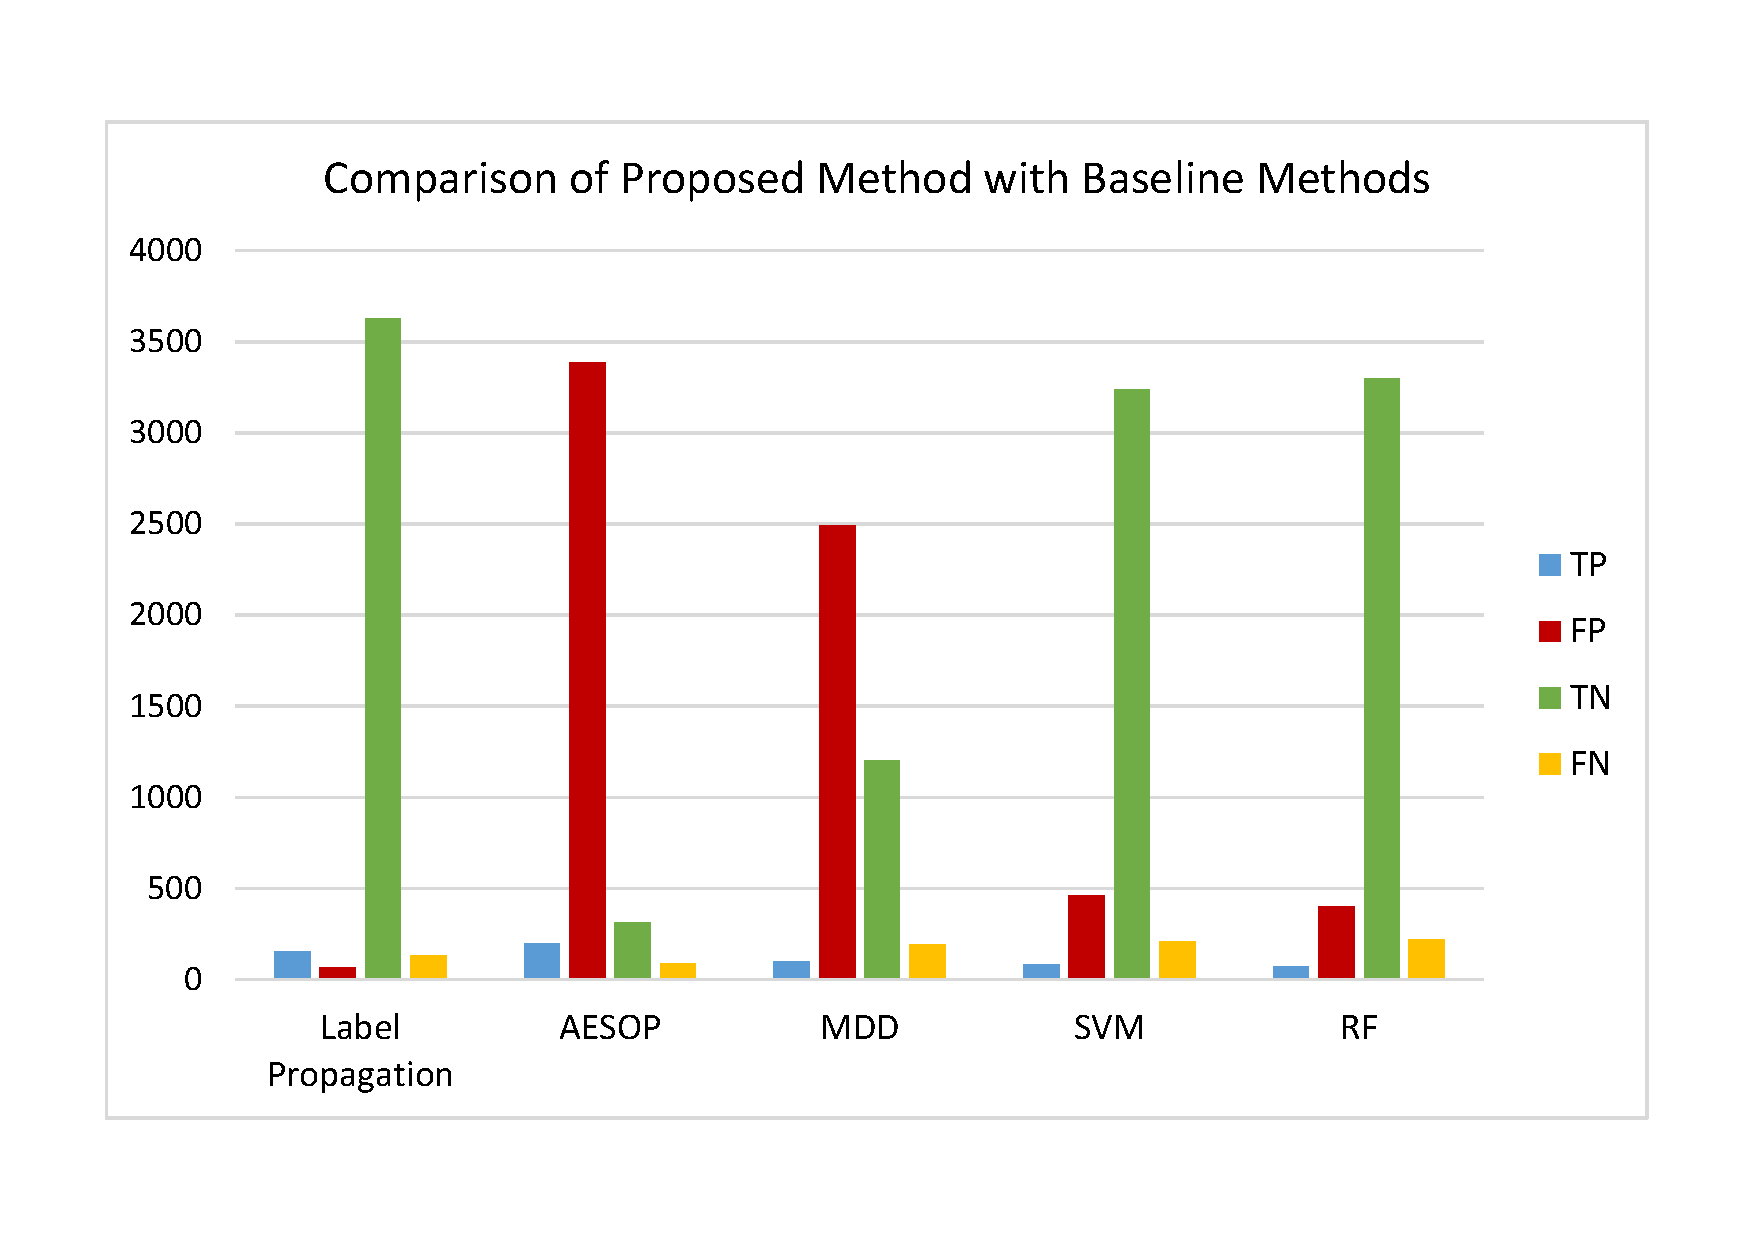
\includegraphics[width=4in]{img/chap2/ResultComparison.pdf}
\caption{在大规模现实数据上算法的性能对比}
\label{fig_ResComparisonWithBaseline}
\end{figure}

\subsubsection{交叉验证}
交叉验证(Cross Validation)是指在某种意义下将原始数据进行分组,一部分做为训练集(Train set),另一部分做为验证集(Test set),首先用训练集对分类器进行训练,再利用测试集来测试训练得到的模型(Model),以此来做为评价分类器的性能指标。通过大量数据集以及不同学习技术进行的大量试验表明10折是获得相对较好误差估计的恰当选择,因此在本实验中使用10折交叉验证(10-fold Cross Validation),将数据集分成十份,轮流将其中的9份作为训练数据,剩余1份作为测试数据,进行试验。每次试验都会得出相应的正确率(或差错率)。10次的结果的正确率(或差错率)的平均值作为对算法精度的估计。在每一次验证中,将测试集的标签设为0(即未标记),标签概率均为0.5(即样本被预测为恶意软件和良性文件的概率是相等的)。基于10折交叉验证的数据结果对比如盒图\ref{fig_Boxplot}所示,图中每个数据盒子中的缺口代表了中位数的95\%置信区间。从图中可以看出,本章提出的基于标签传播的恶意软件检测算法与其他算法相比在检测准确率上能够获得明显的改进和提升。

\begin{figure}[!ht]
\centering
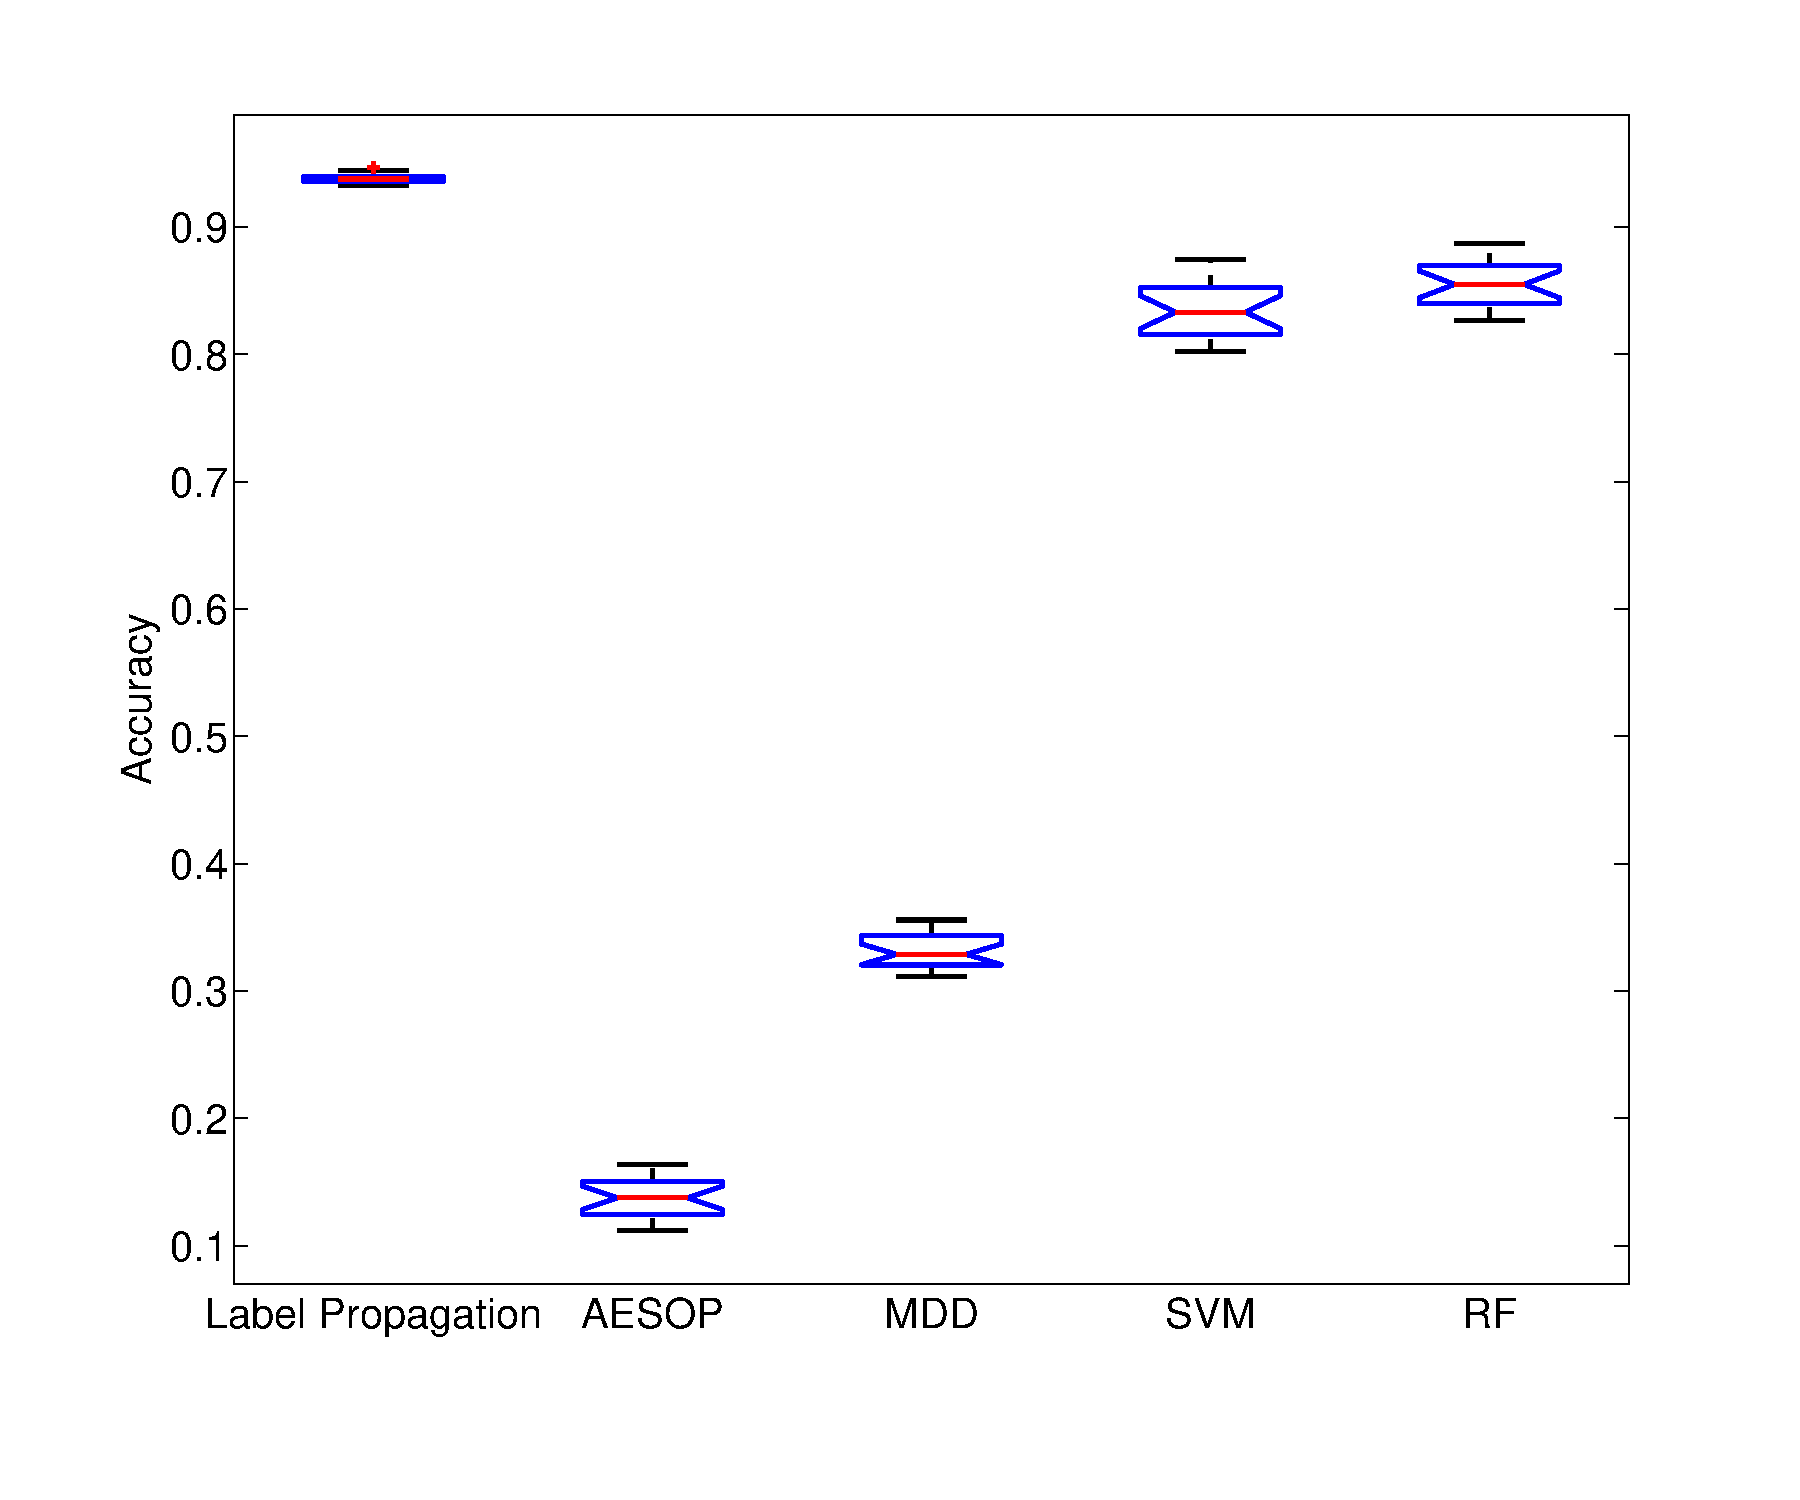
\includegraphics[width=4in]{img/chap2/Boxplot.pdf}
\caption{10折交叉验证准确率对比}
\label{fig_Boxplot}
\end{figure}

\section{本章小结}
本章主要研究了文件样本之间关联关系在恶意软件检测中的相关应用,提出了一种基于标签传播的恶意软件检测方法。采用共存关系作为文件样本之间的关联关系,运用了Jaccard相似度算法来衡量文件样本之间的相似度,在此基础上通过选取每个文件样本的$k$个近邻作为邻接节点来构建文件样本的关联关系图。标签传播算法是一种将已标记节点的标签信息传递给未标记节点的基于图的半监督学习算法。在文件关联图的基础上,利用标签传播算法学习未标记文件样本的标签信息,发现恶意软件样本。将本章中的算法应用于一个从工业界采集得来的大规模真实数据进行实验,通过与真实的数据进行对比,证明提出的算法具有较高的准确性,能够精准的发现新的恶意软件样本。

在后续的研究工作中,需要进一步研究基于图的恶意软件检测算法,分析文件样本的社交关系以及改进基于图的半监督学习算法,提高恶意软件检测的准确率和可靠性。

\makeatletter
\addtocontents{lof}{\vspace{-10pt}}
\addtocontents{lot}{\vspace{-10pt}}
\makeatother

\iffalse
\bibliography{../bib/thesis.bib}
\fi

\chapter{基于文件社交网络的恶意软件检测方法研究}

\section{相关研究}

\section{系统架构}
基于文件社交网络的恶意软件检测系统架构包含四个主要模块,如图\ref{fig_SysArchitecture}所示。文件列表采集模块(\textit{File List Collector})从用户的终端设备(包括个人电脑,手机和平板等智能设备)采集文件样本,同时提取出文件样本间的关联关系,并转存文件列表以及每个文件的关联关系至文件关系数据库(\textit{File Relation Database})中。文件关联图构造模块(\textit{File Relation Graph Constructor})根据关系数据库构造能够表示文件之间关联关系的文件关联图,在系统框架中起重要的作用。在文件关联图的基础之上,图特征提取和采样模块(\textit{Graph-based Feature Extractor})分析基于图的特征属性,在这些特征属性的基础之上选择一些具有重要的代表性的节点(对应的文件样本)进行人工标记,从图属性的层面提高分类器的准确率水平,使得模型更加健壮。作为系统结构的核心,基于主动学习(Active Learning)的标签传播分类器(\textit{Label Propagation Classifier})根据文件关联图学习未标记样本的标签信息(即恶意或者良性),在学习的过程中主动学习(Active Learning)选择重要的文件样本进行人工标记从而在算法层面上提高标签传播分类器的性能。

\begin{figure}[!ht]
\centering
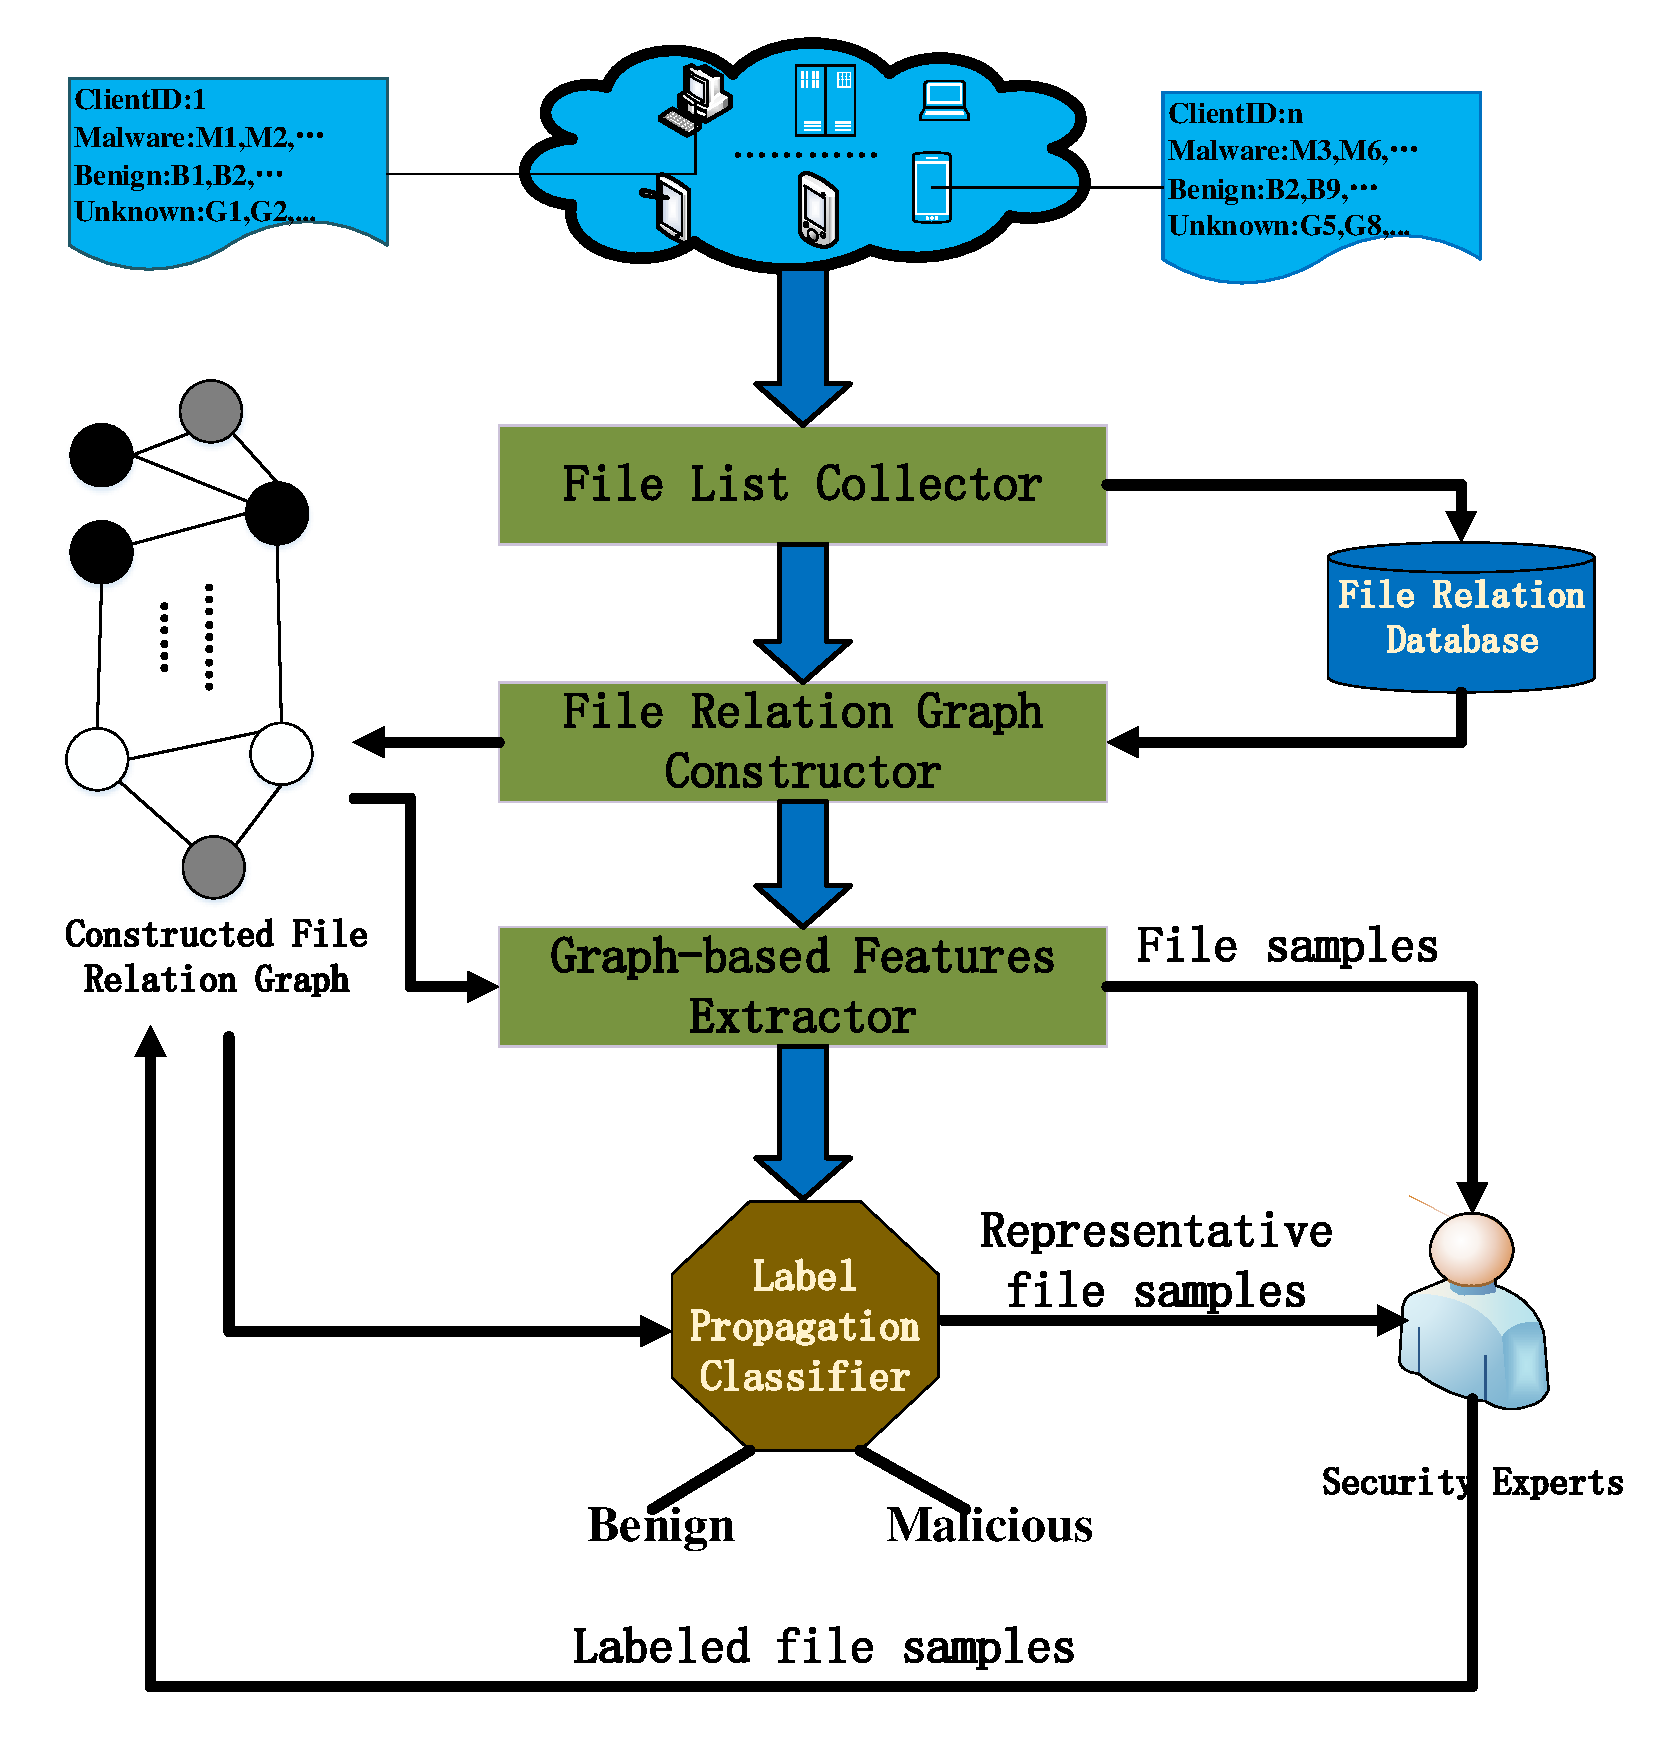
\includegraphics[width=3.5in]{img/chap3/SystemArchitecture.pdf}
\caption{总体框架}
\label{fig_SysArchitecture}
\end{figure}
\section{文件样本社交网络分析}
\subsection{文件关联图}
本章采用上一章中文件关联图的构建算法($k$近邻图)构建文件关联图,图\ref{fig:vis:1}为构建的文件关联图,图\ref{fig:vis:2}和图\ref{fig:vis:3}分别展示了其中一个恶意文件样本和良性文件样本及其它们一跳范围内的关联信息。其中,红色点为恶意软件,绿色点为良性文件,黄色点为未标记样本。
\begin{figure}[!ht]
\centering
\subfigure[文件关联图]{\label{fig:vis:1} 
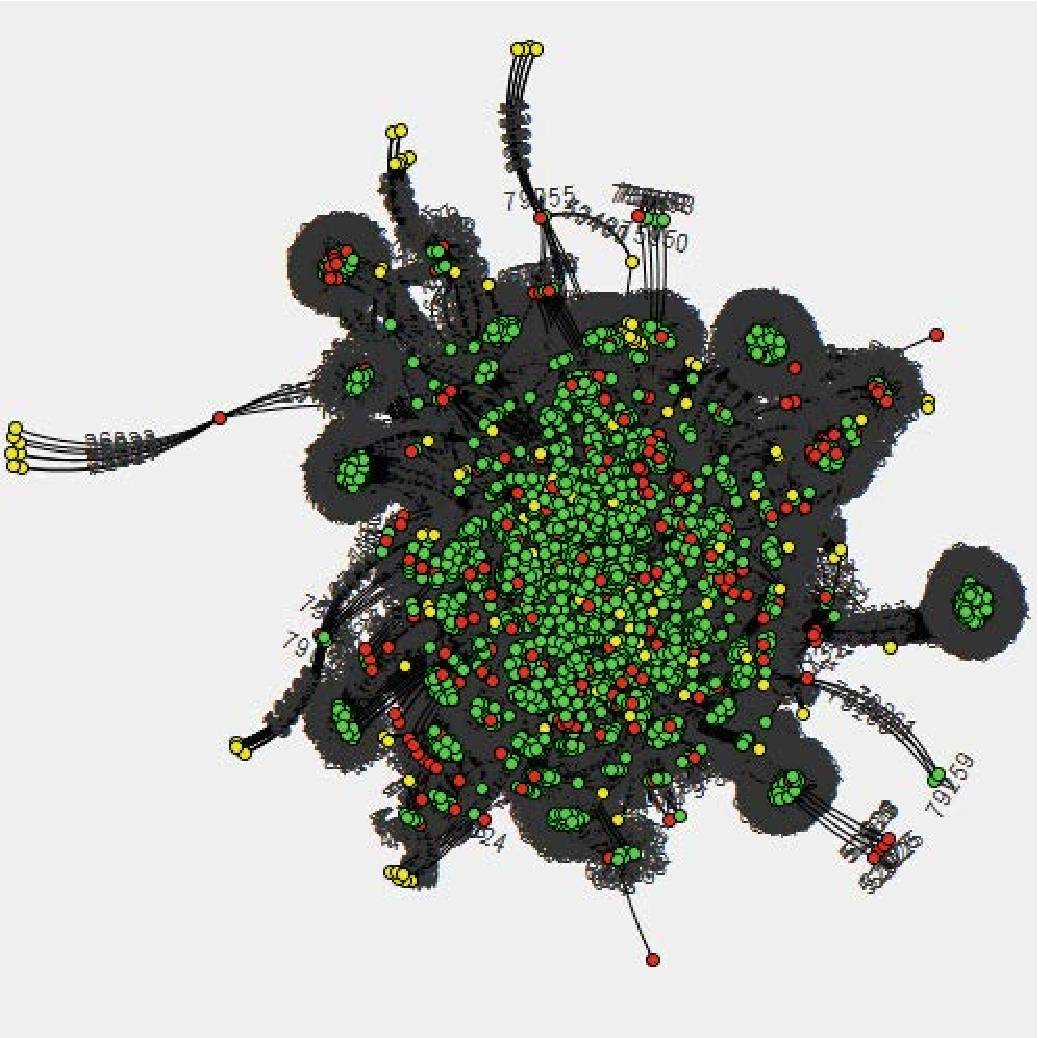
\includegraphics[width=.32\linewidth]{img/chap3/vis1.pdf}}
% \hspace{0.1in}
% \quad
\subfigure[恶意软件关联]{\label{fig:vis:2} 
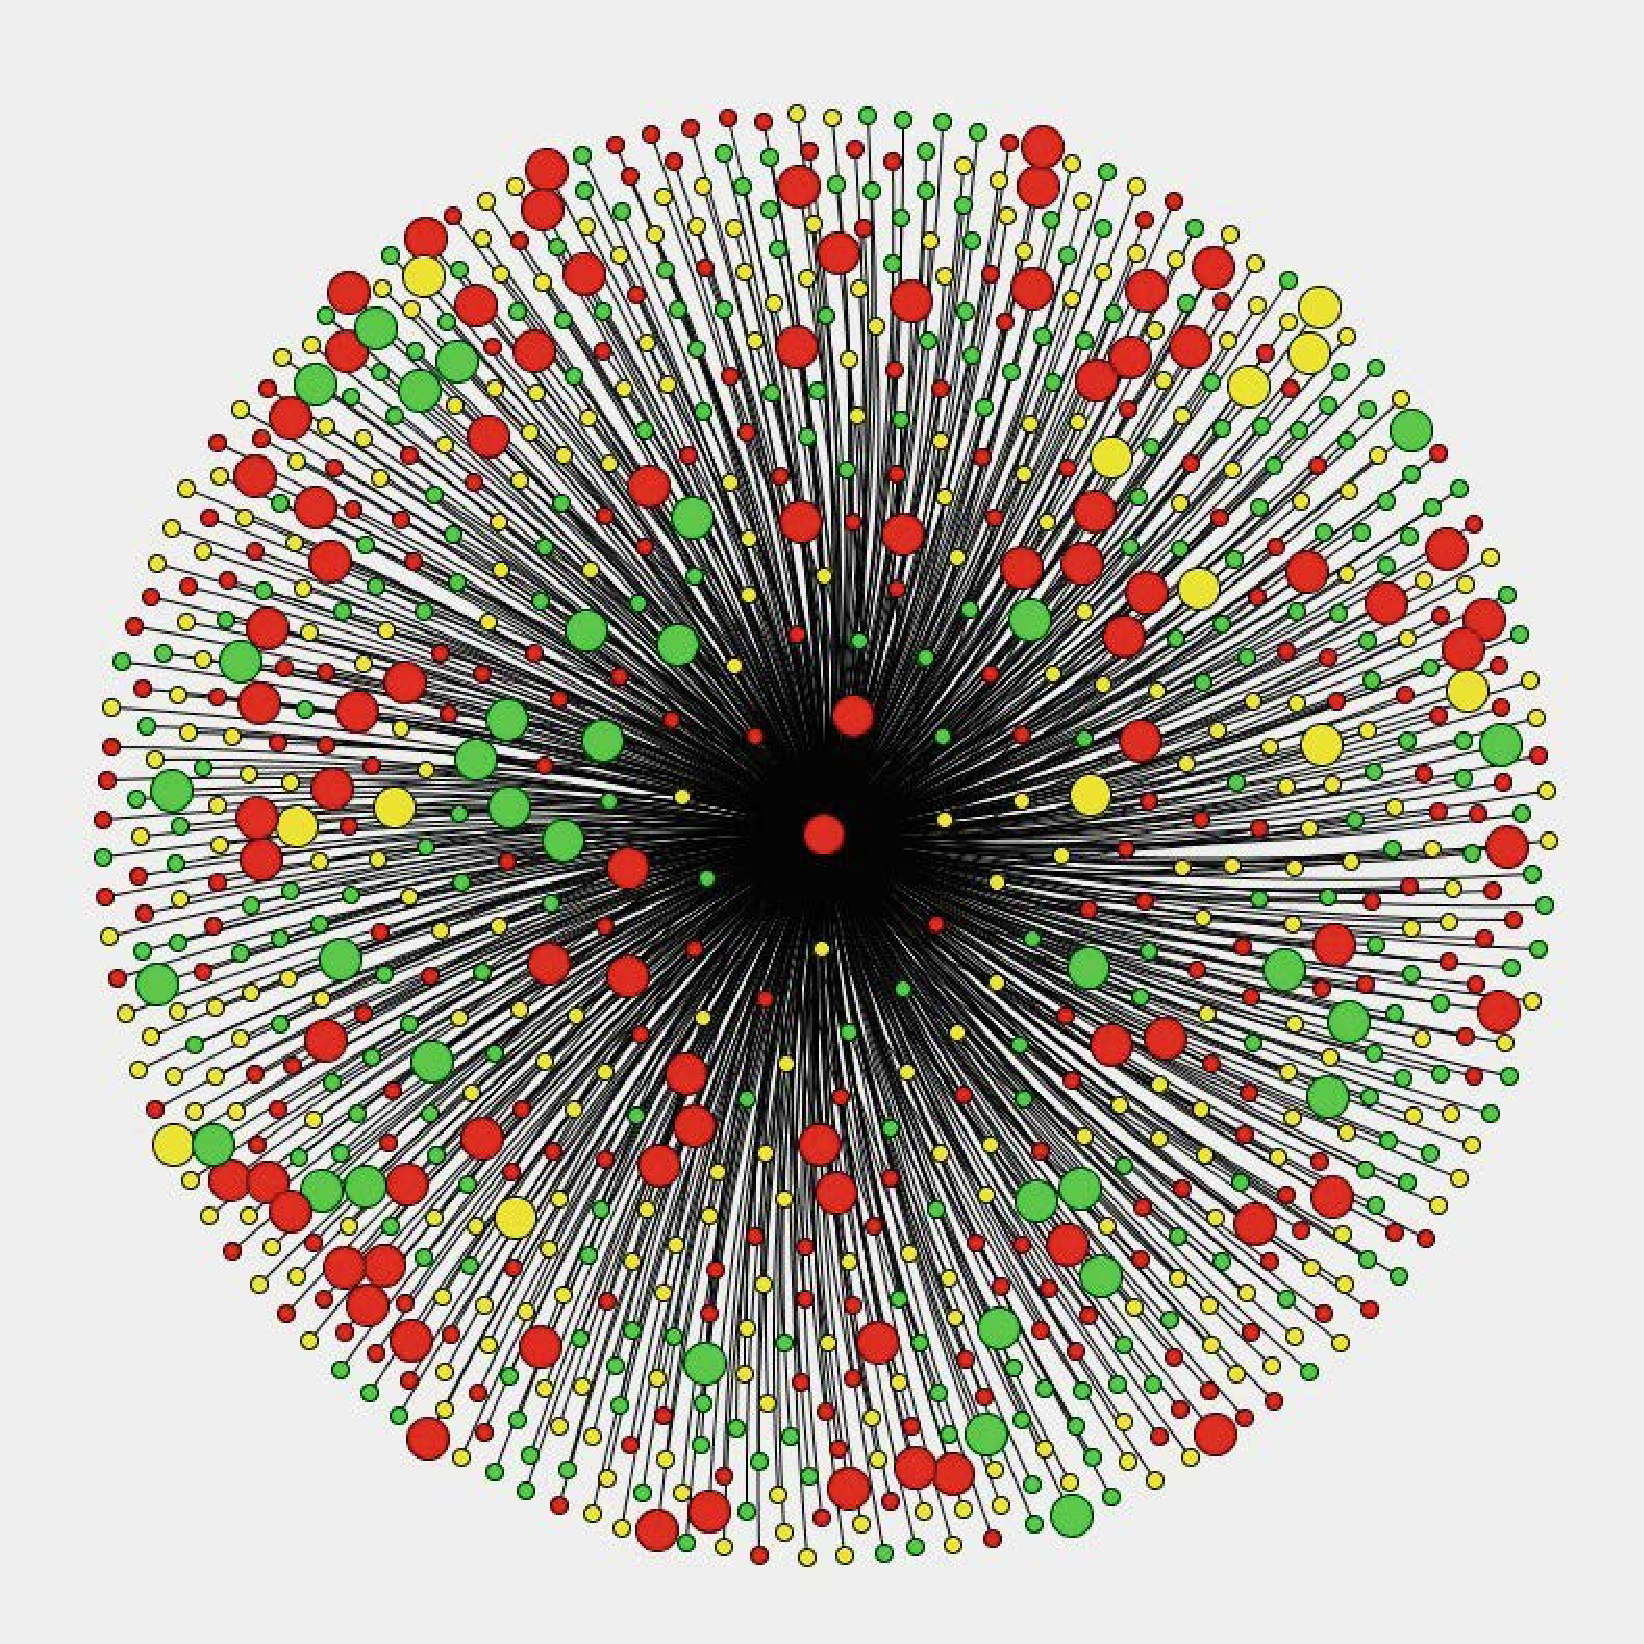
\includegraphics[width=.32\linewidth]{img/chap3/vis2.pdf}}
% \quad
\subfigure[良性文件关联]{\label{fig:vis:3} 
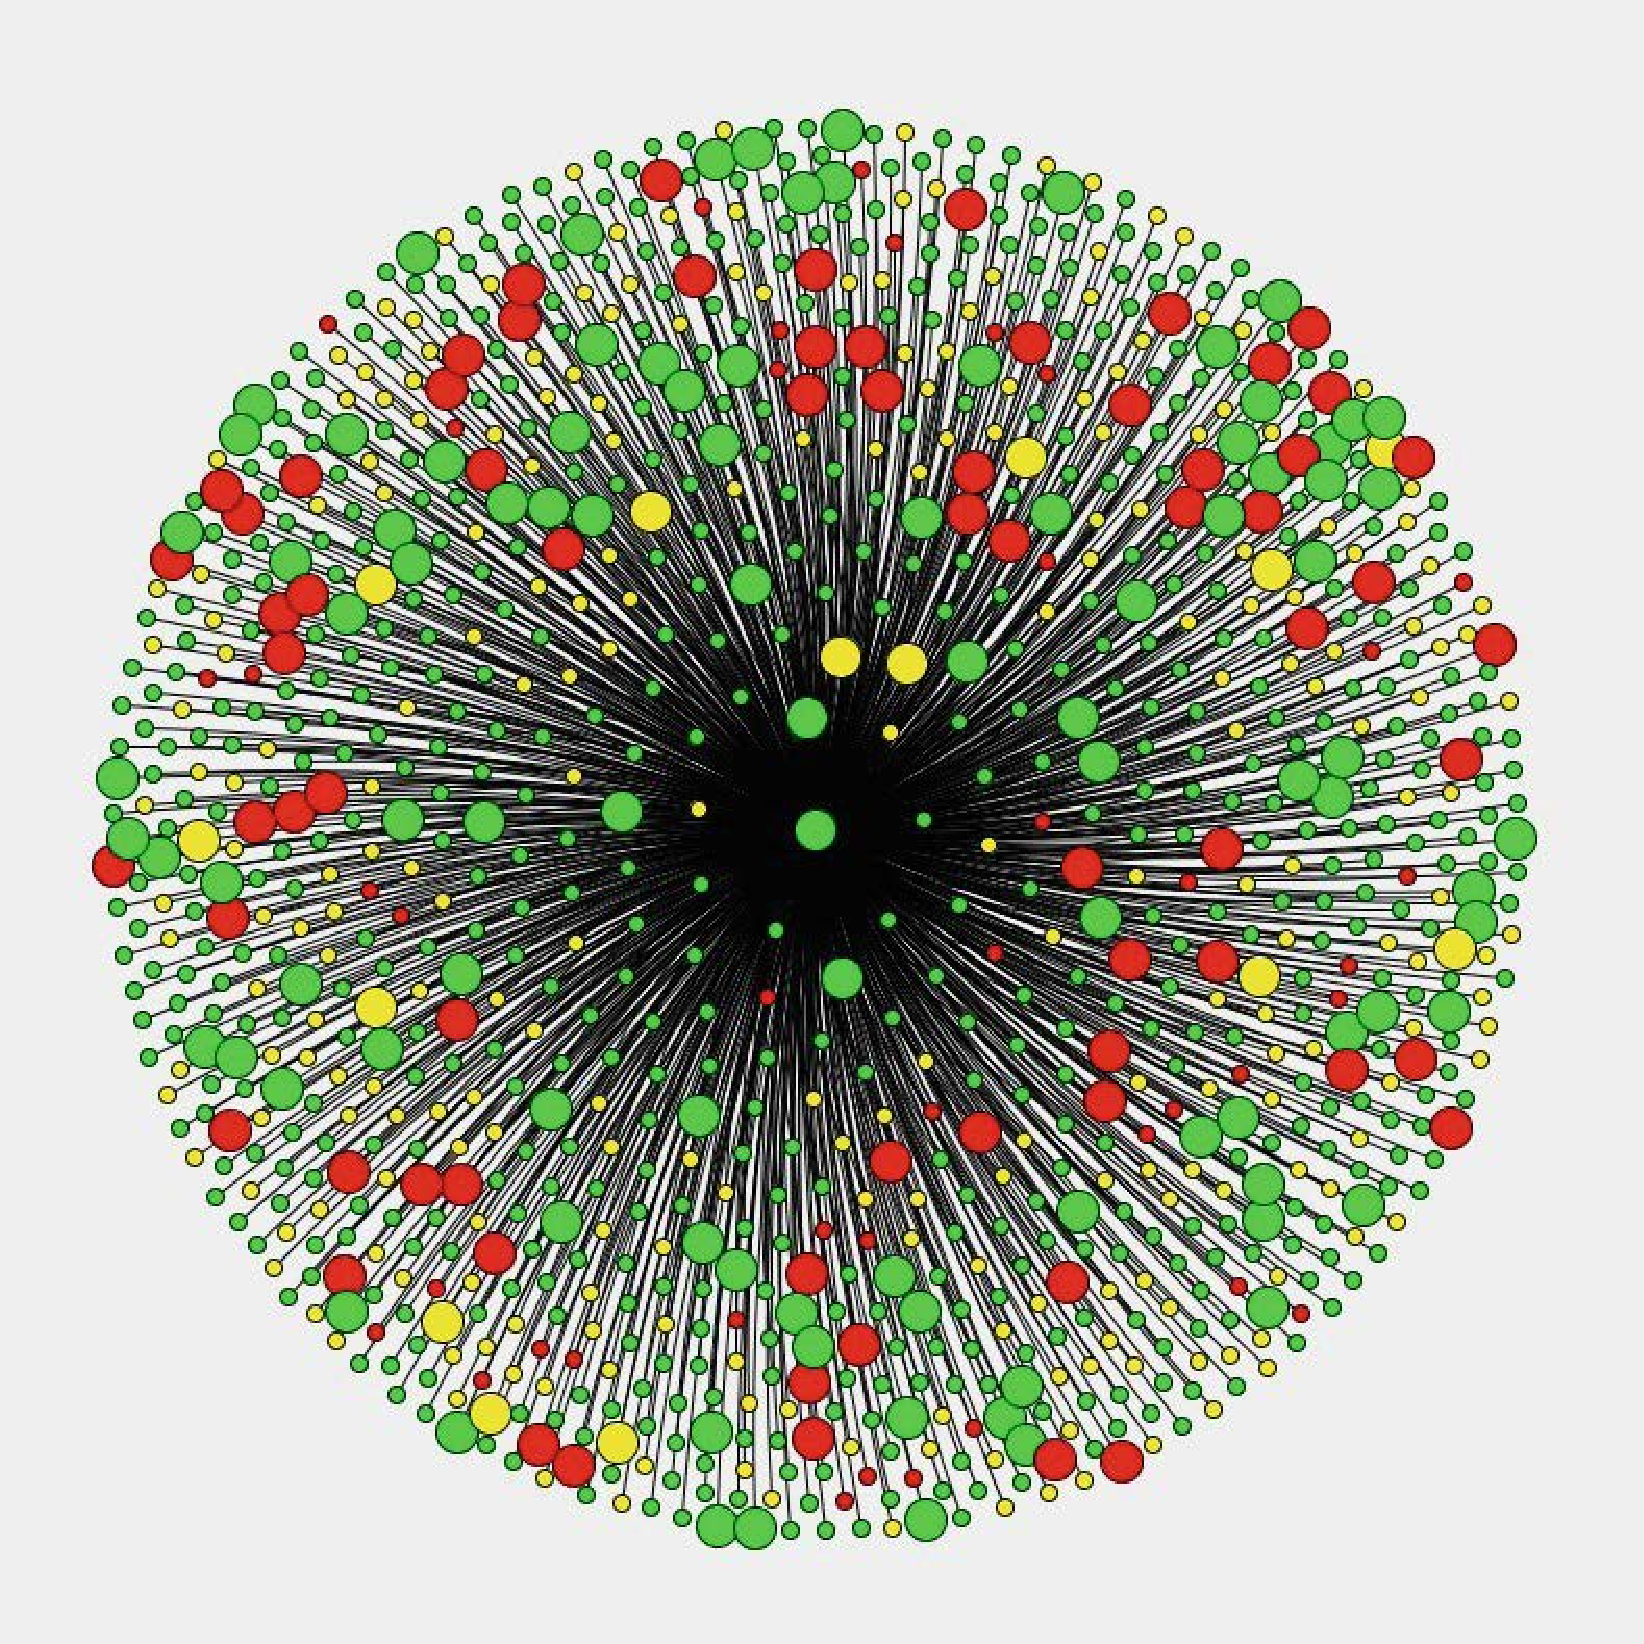
\includegraphics[width=.32\linewidth]{img/chap3/vis3.pdf}}
\caption{文件关联图可视化}
\label{fig:vis}
\end{figure}
\subsection{文件关联网络的特征属性}
\subsubsection{节点度}
在图论中,节点度是指与节点相关联的边的数量,又称为关联度。节点度能够明确的表示节点与其邻居的关联性\cite{diestel2010graph}。在文件关联图中,提出节点的恶意软件度($DoM$)和节点的良性文件度($DoB$)来分别衡量文件与不同类型文件的关联关系,根据公式分别计算:
\begin{equation}
\label{eq:domAnddob}
DoM(v)=\left | \delta_{m}^{v}  \right |, DoB(v)=\left | \delta_{b}^{v}  \right |
\end{equation}
其中,$\left | \delta_{m}^{v}  \right |$是节点$v$恶意邻居节点的数量,$\left | \delta_{b}^{v}  \right |$是节点$v$良性邻居节点的数量。古人云:近朱者赤,近墨者黑。同样的道理,在计算机网络中恶意软件的$DoM$将比$DoB$大,反之亦然。

\subsubsection{局部聚类系数}
聚类系数表示一个图形中节点聚集程度的系数,用于描述网络中节点和其邻居节点之间互相连接的紧密程度,即网络的集团化程度。聚类系数主要分为全局聚类系数、局部聚类系数和平均聚类系数。局部聚类系数表示一个节点的相邻节点形成一个团(完全图)的紧密程度,故本章采用局部聚类系数来计算文件关联图中节点的聚集能力,计算方法为\cite{watts1998collective}:
\begin{equation}
\label{eq:lccUW}
LCC(v)=\frac{2\left | e^{v} \right |}{d_{v}(d_{v}-1)},
\end{equation}
其中$\left | e^{v} \right |$为节点$v$的所有邻居节点之间的边的总数,$d_{v}$为节点$v$的度。这里的局部聚类系数$LCC$在计算时考虑了节点度以及邻居节点之间的边,能够较好的表达无权图中节点的局部紧密程度。而在带权图中,每条边上的权重衡量了每对节点之间的相似度,而在公式\ref{eq:lccUW}的计算中每个邻居节点都被平等对待,没有考虑每对节点之间的相似程度,即两点之间边的权重,因此在带权图中,计算节点的局部聚类系数时需要根据连接至节点的边的权重来计算。Jukka-Pekka Onnela等人\cite{onnela2005intensity}提出了一种基于子图强度的带权图局部聚类系数计算方法,定义为子图中边权重的几何均值:
\begin{equation}
LCC(v)=\frac{1}{d_{v}(d_{v}-1)}\sum_{i,j \in N(v)}(\hat{w}_{vi}\hat{w}_{vj}\hat{w}_{ij})^{1/3},
\end{equation}
其中,$N(v)$是节点$v$的邻居节点集合,$\hat{w}_{vi}$是经过公式\ref{eq:LCCnormalize}归一化的边权重。
\begin{equation}
\label{eq:LCCnormalize}
\hat{w}_{vi} = \frac{w_{vi}} {max(w)}
\end{equation}

每个人对于电脑、手机等智能设备都有不同的用途和使用习惯,因此也会安装或者拷贝不同类型的程序和文件。举例来说,办公室文员经常需要使用Word、Excel等办公事务处理类的应用软件,而这一类的软件彼此之间也都会有较高的关联性和相似度,这就使得这些软件可以被划分为具有高关联性和相似度的群体,因此办公软件``'Word''会拥有较大的局部聚类系数$LCC$。类似的,在恶意软件中,病毒``下载者''(Trojan-Downloader)通过用户的计算机从其作者指定的URL地址下载一个或多个的病毒文件并在本地运行,这些下载得到的病毒文件以及对应的``下载者''病毒有较高的共存关系和相似性,所以``下载者''病毒的局部聚类系数会较大。图\ref{fig:lcc}对比了应用程序``Word''和``Photoshop''在局部聚类系数属性上的不同。

\begin{figure}[!ht]
\centering
\subfigure[Word]{\label{fig:lcc:word} 
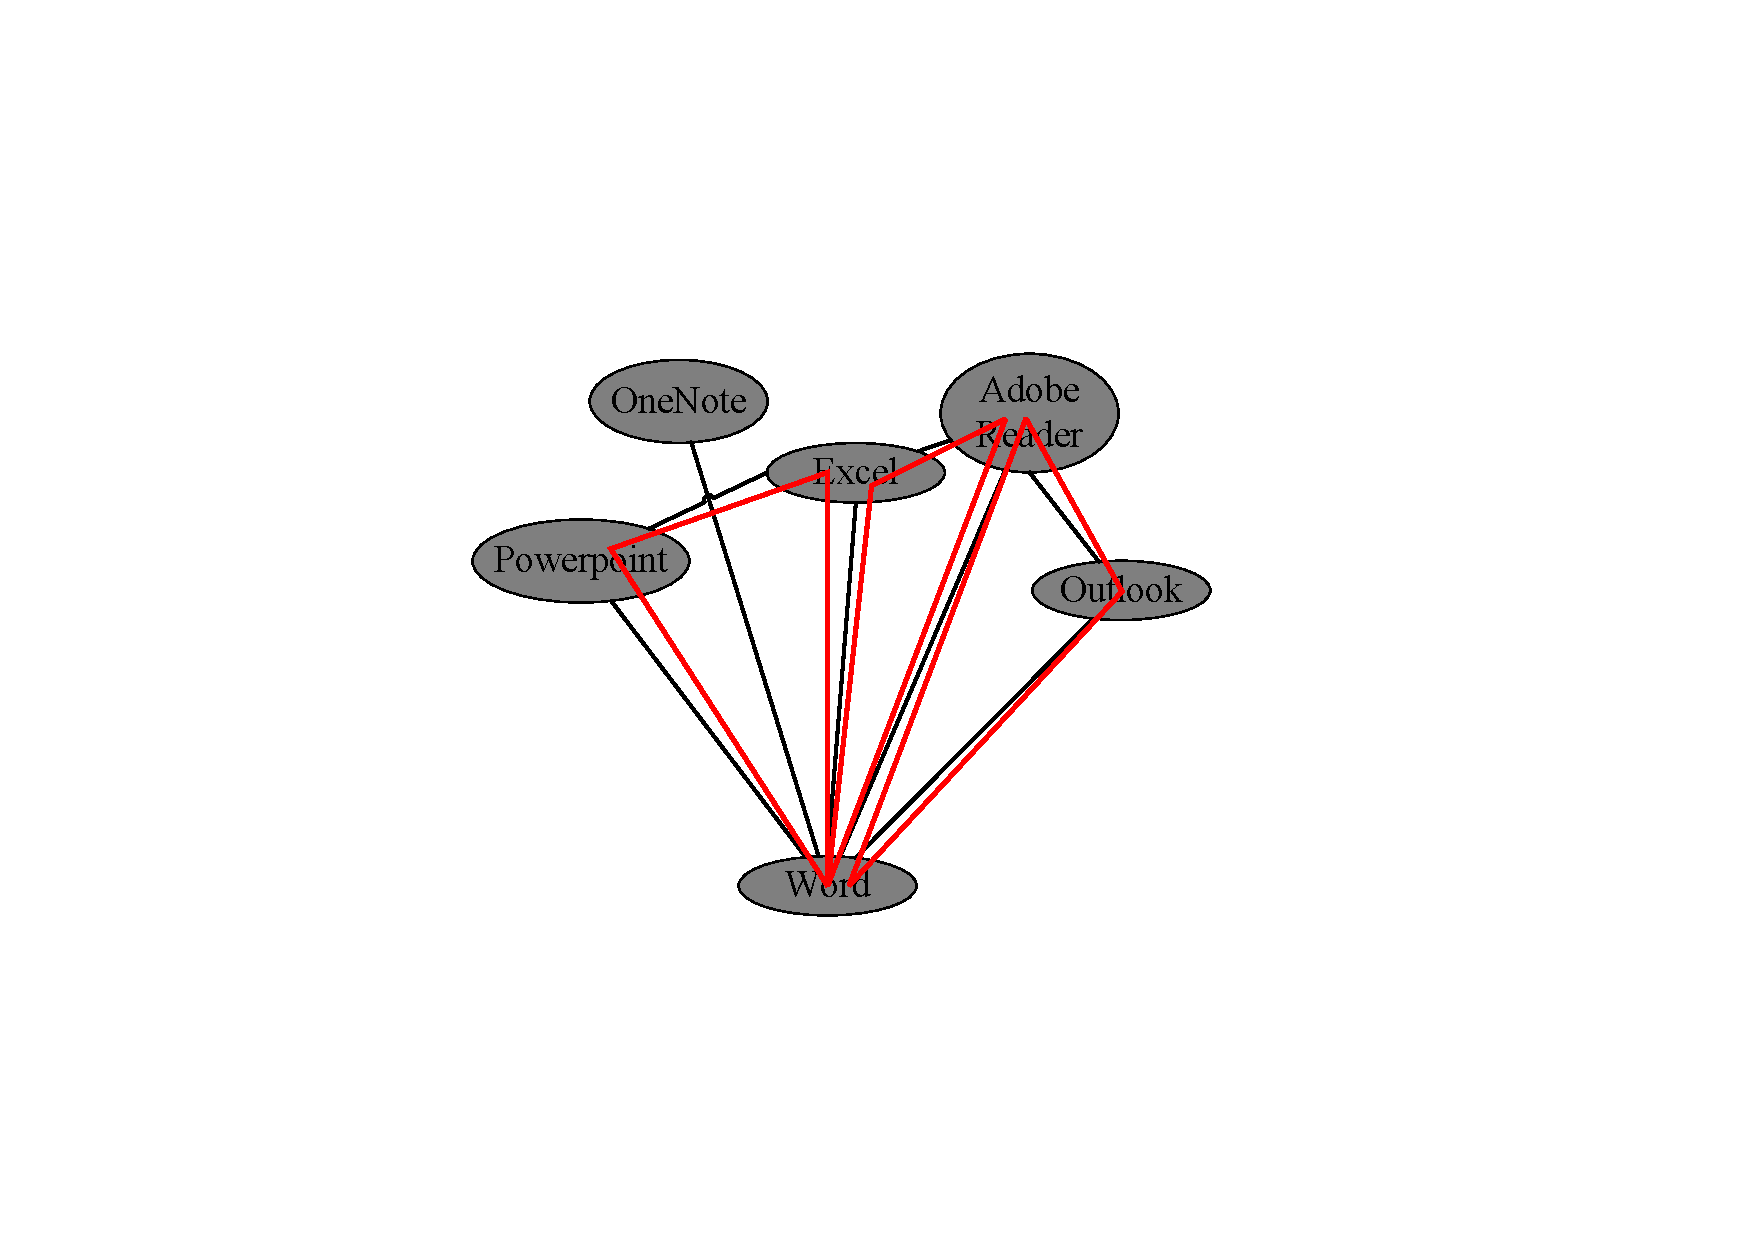
\includegraphics[angle=270, width=.45\linewidth]{img/chap3/LCC.pdf}}
% \hspace{0.1in}
\quad
\subfigure[Photoshop]{\label{fig:lcc:ps} 
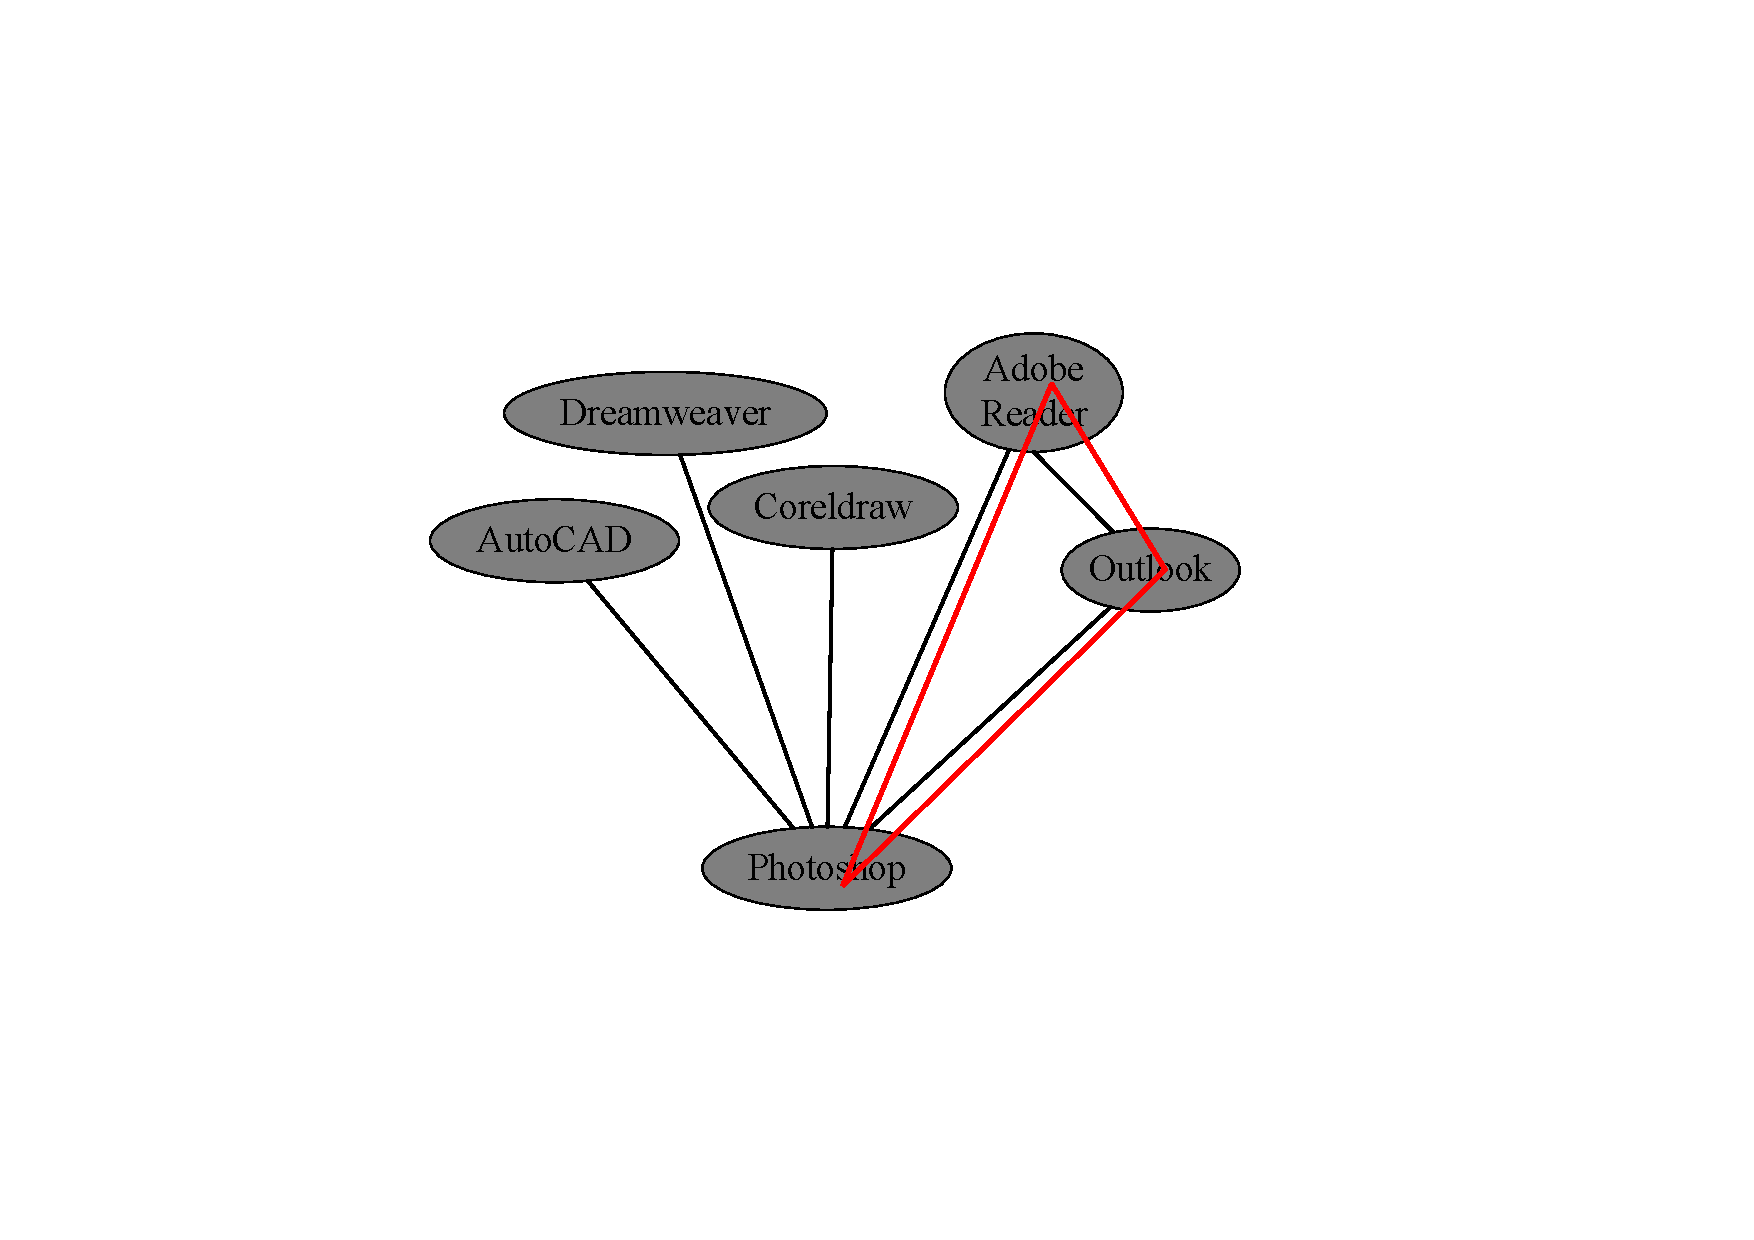
\includegraphics[angle=270, width=.45\linewidth]{img/chap3/LCC_low.pdf}}
\caption{``Word''和``Photoshop''局部聚类系数对比}
\label{fig:lcc}
\end{figure}

\subsubsection{度中心性}
度中心性(Degree Centrality)是在网络分析中刻画节点中心性(Centrality)的度量指标。一个节点与越多的节点发生直接联系,节点的节点度就越大,就意味着节点的度中心性越高,那么这个节点就处于中心地位,在网络中就越重要\cite{scott2012social}。
\begin{equation}
DC(v)=\frac {d_{v}} {n-1}
\end{equation}
其中,$n-1$为节点$v$可能连接的最大节点数,$n$为图中节点的数量。

\subsubsection{接近中心性}
接近中心性反应了节点在网络中与其他节点之间的接近程度,体现了节点对图的全局认识程度。具有较高接近中心性的节点能够比其他节点更快速的触及整个图。
\begin{equation}
CC(v)=\frac {n-1} {\sum_{u \neq v}^{n}g(u,v)}
\end{equation}
其中,$g(u,v)$是节点$u$和$v$之间的最短路径,$n$为图中节点的数量。

\subsubsection{中间中心性}
中间中心性体现了一个节点在图中的地位。中间中心性的概念由Linton于1977年提出,用来衡量一个人在社交网络中控制他人信息交流的能力\cite{freeman1977set}。如果一个节点处在许多节点互联的路径上,可以认为此节点处于重要地位,因为该节点具有控制其他节点交互的能力,其他节点之间的交互需要通过该节点才可以进行。出现在很多其他节点之间最短路径上的节点将比其他的节点拥有更大的中间中心性。节点$v$的中间中心性可以根据公式\ref{eq:bc}计算,$\delta_{st}$是从节点$s$到节点$t$的最短路径总数,$\delta_{st}(v)$为从节点$s$到节点$t$的最短路径中经过节点$v$的路径个数,$n$为图中节点的总数。
\begin{equation}
\label{eq:bc}
BC(v)=\frac {1} {(n-1)(n-2)}\sum_{s \neq v \neq t \in V} \frac {\delta_{st} (v)} {\delta_{st}}
\end{equation}

\subsection{基于图属性的文件采样}
根据文件社交网络的关系以及每个文件所处位置可以看出,每个文件的重要性是不同的,重要性较高文件的邻居通过这些文件产生关联关系。因此,根据图的特征属性从大量的未标记文件集中选取具有代表性的重要的文件进行标记对于提高恶意软件检测的准确率和性能是十分重要的。本章选择度中心性(DC)、局部聚集系数(LCC)和接近中心性(CC)作为衡量文件重要性的因子,定义文件的重要性为:
\begin{equation}
importance(v_{i}) = \frac {DC(v_{i}) * LCC(v_{i})} {CC(v_{i})}
\end{equation}
该值越大,文件的重要性越大。根据重要性对未标记文件进行降序排序,选取前$k$个文件作为采样样本交由安全专家进行标记并加入已标记样本中来训练分类器。

\section{主动学习}
在传统的数据挖掘算法中,学习算法以给定的已标记样本数据集作为训练集进行训练学习。然而在很多现实的应用中,往往面临的情况是大量的未标记样本和极少量的已标记样本,而且未标记样本比已标记样本更加容易获取。对样本进行标记工作的成本是高昂的和困难的,需要花费大量的人力、物力和财力。Zhu等人研究表明\cite{zhu2005semi},对于训练样本的准确标记不仅需要数据的领域知识和领域专家,而且样本标记工作所需的时间是获取数据所花费时间的10倍以上。根据PAC学习理论,已标记样本的数量越多,算法的泛化误差越小,因此稀少的已标记样本使得现有的监督学习算法的应用能力大大降低。主动学习(Active Learning)算法被提出以有效地解决这类问题。主动学习算法模拟了人类的学习过程,通过选择重要的未标记样本进行标记并加入训练集,迭代学习来提高分类器的学习能力。
\subsection{相关概念}
主动学习是最早由Angluin等人在1988年提出\cite{angluin1988queries},其主要的思想根据数据分布情况,主动选择对分类器模型有重要意义的样本,交由领域专家进行人工标注并把这些样本加入到已标注的训练集中,通过反复的迭代学习训练,使得分类器拥有更好的泛化能力和分类准确率。

主动学习算法一般包括以下两个部分:
\begin{asparaenum}
\item 学习引擎(Learning Engine)。学习引擎在已标记样本集上训练一个分类器,当分类器的准确率或某一度量标准满足条件时结束训练并输出结果。
\item 采样引擎(Sampling Engine)。采样引擎根据学习引擎分类器的分类结果和一种样本选取策略在未标记样本集中选取样本,将样本交由领域专家进行人工标记,并在标记完成后将样本加入到已标记样本集中。
\end{asparaenum}

学习引擎和选择引擎进行循环交替,经过多次循环之后学习引擎中分类器的性能逐渐提高,并在分类器达到一定的性能条件后终止。算法\ref{alg:activelearning}以伪代码的形式描述了主动学习算法的流程。

\begin{algorithm}[!ht]
\caption{主动学习算法伪代码描述}
\label{alg:activelearning}
\begin{algorithmic}[1]
\Input 已标记样本集$L$,未标记样本集$U$,学习引擎$LE$,采样引擎$SE$
\Output 学习引擎$LE$
\Repeat
\State $LE.train(L)$\Comment{在已标记样本集上训练分类模型}
\State $T=LE.predict(U)$\Comment{}
\State $Q=SE.query(U, T)$
\State $Label(Q)$
\State $L=L+Q$
\State $U=U-Q$
\Until {性能条件$Condition$满足}
\end{algorithmic}
\end{algorithm}

采样引擎是整个主动学习过程的核心,根据采样引擎的不同,主动学习算法可分为三类:
\begin{asparaenum}
\item \textbf{成员查询综合(Membership Query Synthesis)}。成员查询综合是主动学习最早被提出的采样方案\cite{angluin1988queries}。算法通过学习器来生成一个样本,并交由专家进行标注。该方法的缺点是忽略了样本集的实际分布情况,有可能生成了人类专家无法标注的样本。
\item \textbf{基于流的主动学习(Stream-based)}。如图\ref{fig:al:stream}所示,基于流的主动学习从真实的样本空间中抽取样本,由选择算法决定是否需要将其交给专家进行标注,若不需要标注则舍弃。这种采样策略通常需要设定一个评价标准来对样本进行评估(例如一个固定的阈值),缺乏对不同应用场景的普适性。同时,算法过程中每次仅选取一个样本与阀值进行比较,忽略了与其他未标记样本的对比。
\item \textbf{基于池的主动学习(Pool-based)}。基于池的主动学习算法将未标记样本集看作一个``池'',每次从池中抽取最有价值的样本进行人工标注。基于池的主动学习解决了上述两种方法的缺点和不足,因此是当前研究最多、应用最广泛的样本抽取方法。图\ref{fig:al:pool}为基于池的主动学习算法过程。
\end{asparaenum}

\begin{figure}[!ht]
\centering
\subfigure[基于流的主动学习]{\label{fig:al:stream} 
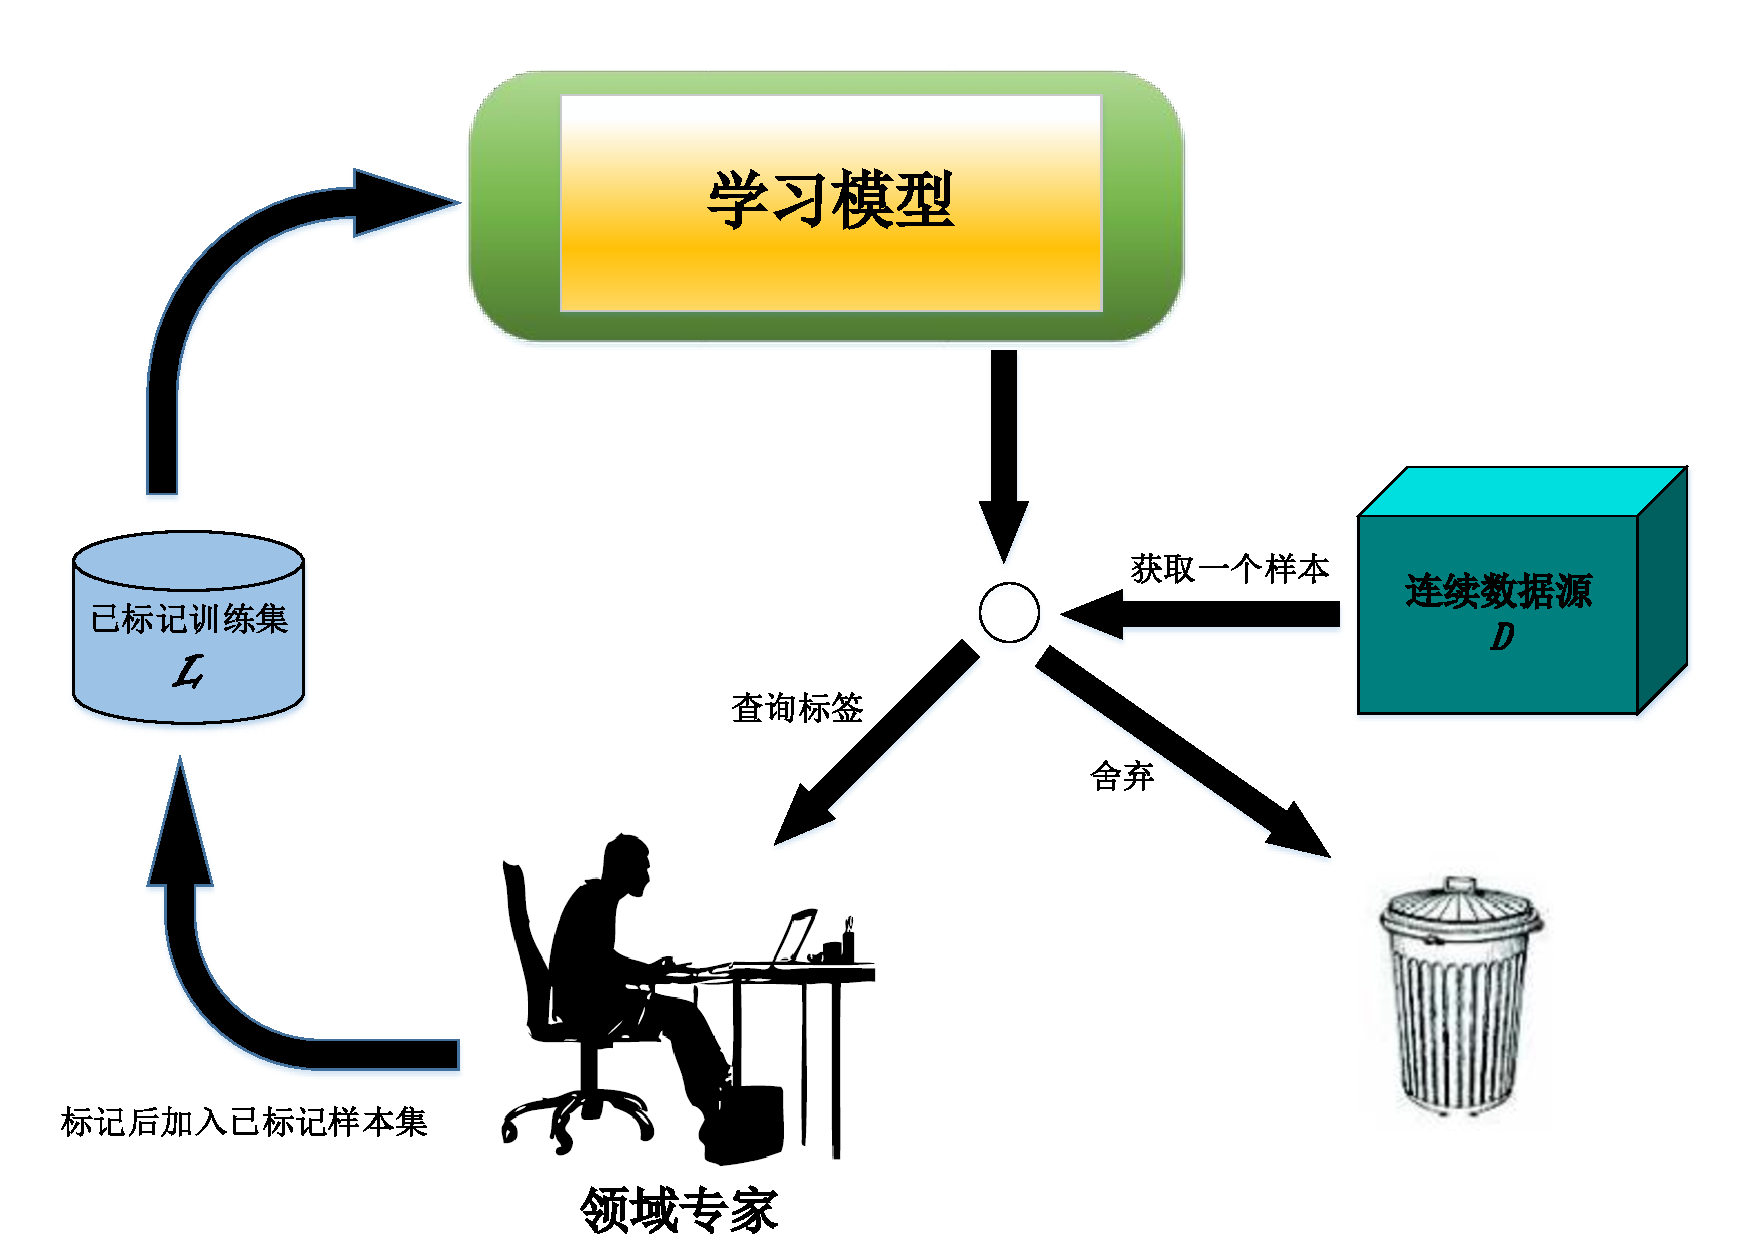
\includegraphics[width=.5\linewidth]{img/chap3/Stream_AL.pdf}}
\quad
\subfigure[基于池的主动学习]{\label{fig:al:pool}
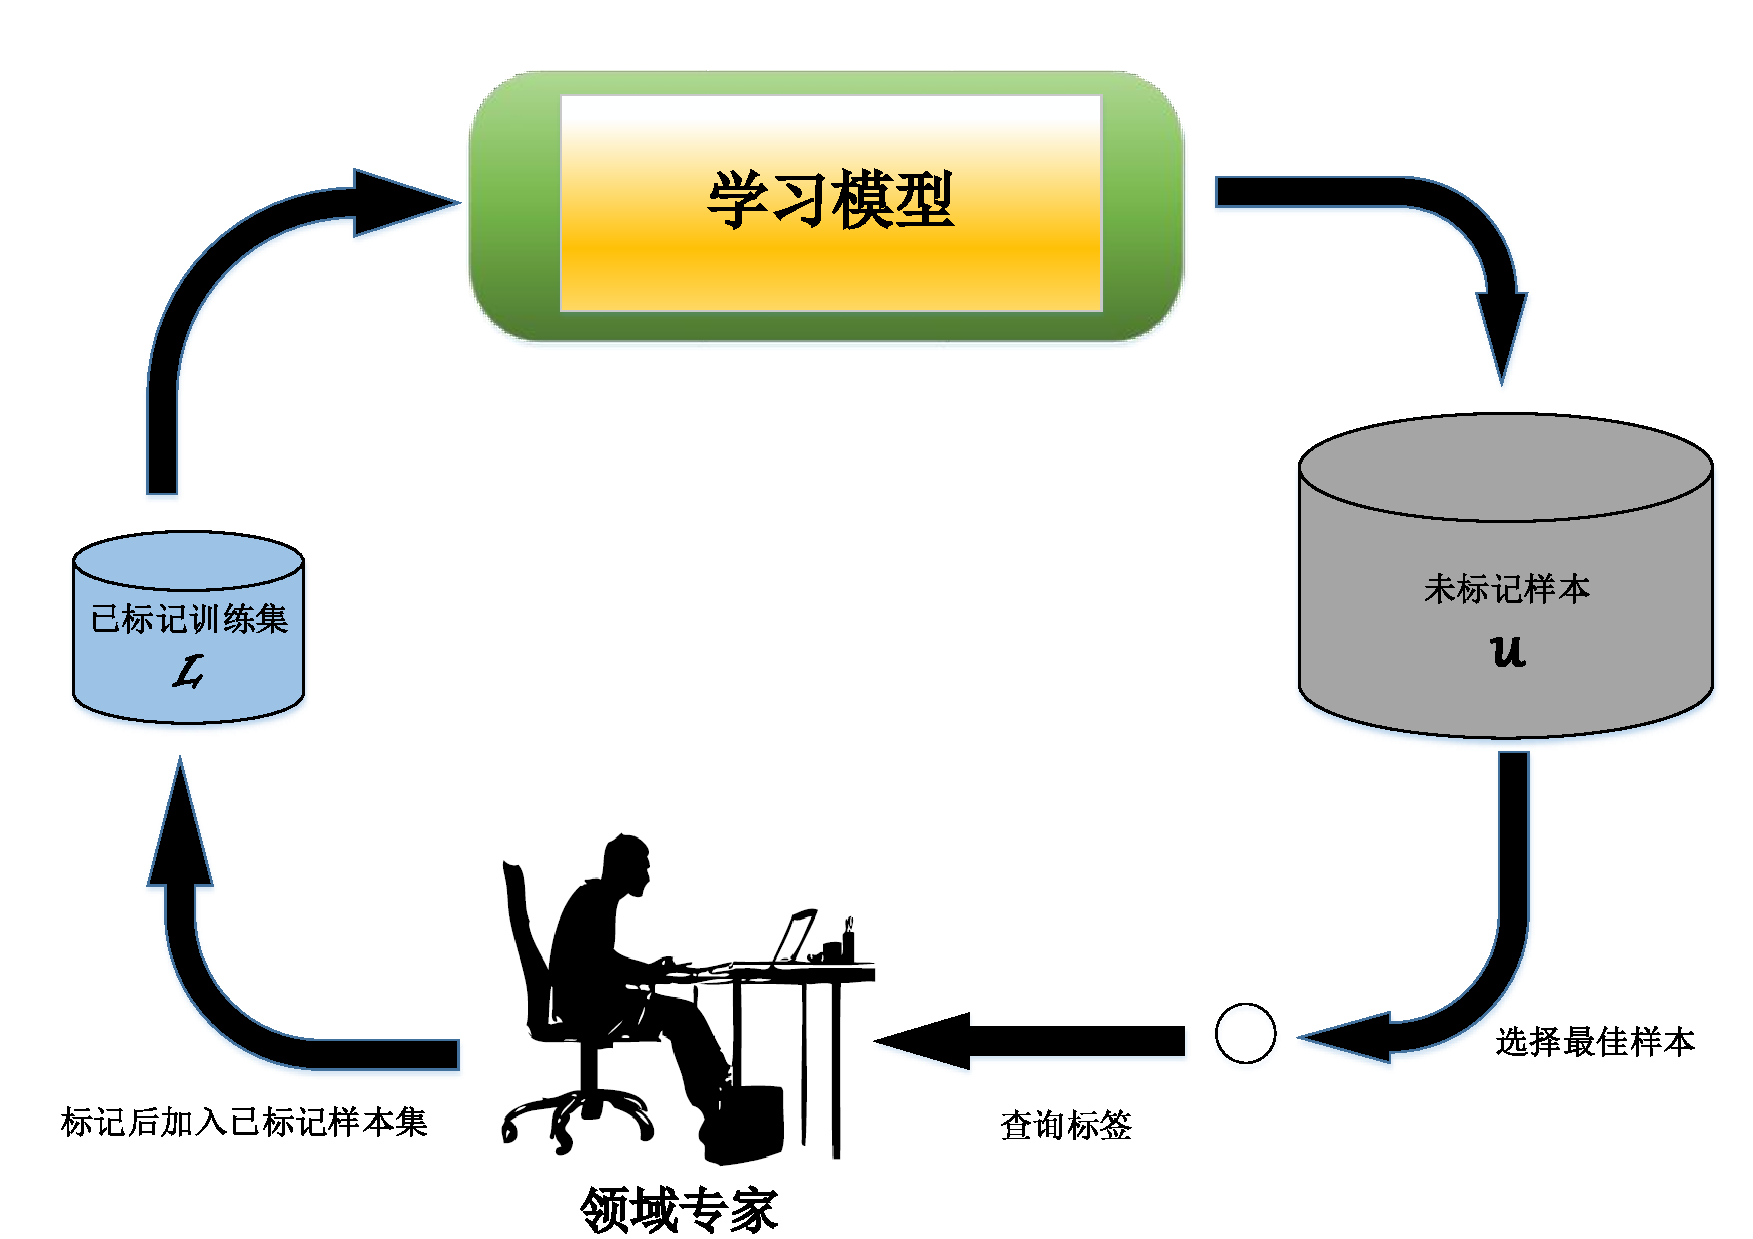
\includegraphics[width=.5\linewidth]{img/chap3/Pool_AL.pdf}}
\caption{主动学习示意图}
\label{fig:al}
\end{figure}

\subsection{主动学习算法采样策略}
近年来,众多的学者和工作聚焦于主动学习算法的研究,尤其是对样本选择算法的研究,希望能发掘出最有意义最具代表性的样本加入训练样本集。在上一节中,我们介绍了主动学习算法中采样方法的三种类型,其中基于池的主动学习算法是目前研究和应用最广泛的样本选择方法。因此,本章主要按照基于池的主动学习算法展开,根据样本选择标准的不同,主要介绍基于不确定性缩减、基于版本空间缩减和基于期望误差缩减三种样本选择策略。
\begin{asparaenum}
\item \textbf{基于不确定性缩减}。基于不确定性缩减的样本选择是目前研究较多的一种基于池的样本选择方法。这种选择方法选择当前分类器最无法确定标签的样本并交由专家进行标记。这种方法对于概率学习模型来说最简单适用。例如,对于二分类问题的概率模型来说,基于不确定性缩减的采样策略将选取那些后验概率接近0.5的样本\cite{lewis1994heterogeneous}。对于分类器来说,最无法确定标签的样本也是分类器最有可能产生分类错误的样本,选择这类样本进行人工标记,不仅能够有效减少人类专家的标注工作,也能较好地提高分类器的准确度和泛化能力。根据分类器模型的不同,衡量样本不确定性的方法和角度也有不同,因此采样策略也会不同,目前常用的方法包括最小边界、最低确定度、最小边缘、最大信息熵等。信息熵(Entropy)\cite{shannon1948math}是编码分布所需信息量的信息论度量,因此通常被认为是机器学习中不确定性或不纯度的度量:
\begin{equation}
x_{H}^{*}=\underset{x}{\arg\max}-\sum_{i}P_{\theta }(y_{i}|x)\log P_{\theta}(y_{i}|x)
\end{equation}
其中,$y$为所有的标签集合。基于信息熵的采样策略受到了广泛的研究和应用\cite{culotta2005reducing,hoi2006large},适用于各种复杂模型和多类别问题,在自然语言处理、文本分类等领域均有较好的性能。基于不确定缩减的采样策略可以应用于多种分类器模型,如逻辑回归(Logistic Regression)、隐马尔科夫模型(Hidden Markov Model)以及支持向量机(Support Vector Machine)等,在多数问题上都能获得较好的性能。
\item \textbf{基于版本空间缩减}。版本空间是概念学习中与已知训练集一致的所有假设(Hypothesis)的子集集合,因此学习器所需要训练的目标假设肯定也包含其中。基于版本空间缩减的主动学习样本选择方法的目的就是选择那些能够最大程度地缩减版本空间的样本进行标记。委员会投票选择算法(Query By Committee, QBC)是一种典型的版本空间缩减的样本选择方法。首先,从当前的版本空间中随机地选择$C$个不同的假设构成一个委员会$Committee=\{\theta^{(1)},...,\theta^{(C)}\}$,委员会中的每个假设对所有未标记样本进行分类投票,选择各个假设分类结果差异最大的样本交由专家进行标记。换句话说,在当前的训练集上构建多个分类器模型,运用这些模型来预测未标记样本,并选择分类结果不一致性的样本进行标记。委员会投票选择算法的核心是如何衡量成员对样本的的不一致性程度。作为最早提出的QBC算法\cite{seung1992query},Seung等人采用投票熵作为评价委员会成员分类差异度的标准:
\begin{equation}
x_{VE}^{*}=\underset{x}{\arg\max}-\sum_{i}\frac {V(y_{i})} {C}\log \frac {V(y_{i})} {C}
\end{equation}
其中,$y_{i}$为所有可能的类别,$V(y_{i})$是投票为$y_{i}$的委员会分类器个数,$C$是委员会的分类器个数。McCallum等人将样本分布密度与QBC相结合的EM-QBC算法,引入KL分歧度(Kullback-Leibler Divergence)作为衡量两个概率分布差异程度的标准,计算方法如下:
\begin{equation}
KL(p_{1}(x),p_{2}(x))=-\sum_{i\in L}p_{1}(x_{i})\log\left (\frac {p_{1}(x_{i})} {p_{2}(x_{i})}  \right )
\end{equation}
该算法的主要思想是委员会成员中不一致性程度最大的样本分布区间包含拥有最大信息量的样本。算法将这一区间内的样本交由专家进行标记。另外,委员会的建立策略也是研究的一个重点,Abe采用集成学习中Boosting和Bagging方法提出了Boosting-QBC和Bagging-QBC的委员会建立策略\cite{naoki1998query}。
\item \textbf{基于期望误差缩减}。主动学习的目的是通过选择最优样本进行标记并加入训练来降低分类器的误差和提高分类器的分类准确率。基于期望误差缩减的样本选择方法就是通过减少分类器的误差来直接提高算法的泛化能力。该方法选择使得分类器未来泛化误差最大程度缩减的样本进行标记。具体步骤为:采样算法将每一个未标记的样本都作为候选样本,将其标记后加入已标记样本训练集并训练分类器;对比分类器训练前后的误差变化,选择能够最大程度缩减分类器泛化误差的样本进行标记并加入已标记样本集。Cohn等人\cite{cohn1996active}提出了基于统计学的主动学习算法,采用了模型方差最小化的缩减策略,并在人工神经网络、高斯混合模型和回归模型中加以应用。基于期望误差缩减的方法,主要搜索使期望误差缩减最大化的未标注样例,来减少标注样例的次数并且有效提高分类器的性能,但是这种方法的计算量较大,尤其是数据集合较大的情况下。
\end{asparaenum}

大多数的主动学习算法致力于每次选择一个最优样本进行标记,在标记后重新训练模型并循环这一过程(采样$\rightarrow$标记$\rightarrow$训练)直至达到迭代次数或满足性能优化要求。然而,很多模型的训练优化是复杂而且耗时的,从而反复训练模型的代价是高昂的,而且如此反复的训练模型在实际的运用中也是不现实的,因此提出了批量模式的主动学习算法。批量模式的主动学习不仅能够减少采样冗余,而且还可以增加样本的多样性。Hoi等人通过最大化查询批量样本的费舍尔信息来解释冗余问题\cite{hoi2006large,hoi2006batch}。

主动学习作为解决数据稀缺问题的有效范例,通过领域专家反馈信息优化了分类器的学习效果,降低了监督学习获取数据标签信息的成本,近年来已经受到广泛关注和深入研究\cite{nguyen2004active,muslea2006active}。特别是随着在各种应用领域内图和网络数据的丰富,基于图的主动学习已经受到很多研究的关注\cite{cesa2010active,cesa2010activetreesandgraph,zhao2008scalable}。

\subsection{最大批量网络增益的采样算法}
最大批量网络增益采样是批量模式主动学习的优化采样策略,将代表性和多样性与传统的不确定性标准相结合。代表性和多样性考虑了训练集中的实例之间的相互依存关系,是不确定性标准的两个补充标准。在选择待标记样本时,样本需要具有代表性以能够提高分类器模型的性能,同时也可以具有更大的多样性以降低标记操作的冗余。最大批量网络增益采样结合代表性和多样性两个特点,并通过最大化网络增益来选择批量样本集。

对于未标记样本集$U$中的每个样本$x_{i}$,查询样本的标签信息的个体信息增益通过信息熵计算:
\begin{equation}
H(x_{i})=-\sum_{y}P(y|x_{i})\log P(y|x_{i})
\end{equation}
其中,$P(y|x_{i})$是标签传播算法计算得到的样本$x_{i}$标签分布概率。

根据标签传播算法,查询批次的网络增益通过传播查询本批次中每个样本的个体信息增益至图中其他的未标记样本来计算,因此定义批量网络增益$NG(B)$为:
\begin{equation}
\label{eq:ng}
NG(B)=\sum_{j \in U-B,i \in B}w_{ji}H(i)-\mu \sum_{i,k \in B,i \neq k}w_{ki}H(i)
\end{equation}
其中,第一部分代表了从剩余未标记样本中查询批量样本的信息增益,而第二部分表示批次内样本之间的冗余,$w_{ji}$是节点$j$和$i$之间边的权重,$\mu$为惩罚因子。批量网络增益结合了不确定性(节点信息熵$H(\cdot)$)、代表性(公式\ref{eq:ng}中第一部分)和多样性(公式\ref{eq:ng}中第二部分)。

在主动学习迭代过程的每一步,选择具有最大网络增益$NG(B)$的样本批次来交由领域专家进行标记。定义$W=[w_{ij}]$为图的邻接矩阵,可以将公式\ref{eq:ng}中第一部分的最大化问题转化为在给定$B$大小的情况下最大化分割图中$B$和$U-B$的问题。通过贪心算法可以求解该问题,伪代码描述如算法\ref{alg:ngal}所述。
\begin{algorithm}
\caption{最大批量网络增益采样}
\label{alg:ngal}
\begin{algorithmic}
\Input 未标记样本集$U$, 批量大小$N$
\State $B=\emptyset $  \Comment{初始化$B$为空集}
\Repeat
\State $k={\arg\max}_{i \in U}{NG(B\cup {i})}$
\State $B\leftarrow B\cup {k}$, $U\leftarrow U-{k}$
\Until {$\left | B \right |=N$}
\end{algorithmic}
\end{algorithm}

\section{基于主动学习的标签传播算法}
上一节我们提出了一个基于批量模式的最大网络增益主动学习采样算法,结合标签传播算法的特点选取能够最大化提升标签传播算法性能的节点进行标记。整体算法描述如算法\ref{alg:allp}所示。
\begin{algorithm}
\caption{Label Propagation With Active Learning}
\label{alg:allp}
\begin{algorithmic}
\Input 未标记数据$D_{U}=(x_{l+1},y_{l+1})...(x_{l+u},y_{l+u})$, 标记数据$D_{L}=(x_{1},y_{1})...(x_{l},y_{l})$及类别集$C$
\Output 未标记数据的类别
\Repeat
\State $initial(D_{U}, D_{L})$ \Comment{初始化相似度矩阵$W$和标签传递矩阵$T$}
\For{$i=0; i<l+u; i++$} \Comment{初始化标签矩阵$Y$}
\For{$j=0; j<\left | C \right | ; j++$}
\State $Y_{ij} = p(y_{i},C_{j})$
\EndFor
\EndFor
\Repeat
\State $Y\leftarrow \overline{T}Y$ \Comment{传播标签信息}
\State $clamp(D_{L})$ \Comment{限定已标记数据}
\Until {$Y$ converges}
\State $B=\emptyset$  \Comment{初始化$B$为空集}
\Repeat
\State $k={\arg\max}_{i \in U}{NG(B\cup {i})}$
\State $B\leftarrow B\cup {k}$, $U\leftarrow U-{k}$
\Until {$\left | B \right |=N$}
\Until {the stopping criterion S is satisfied}  \Comment{直至满足迭代停止条件}
\State $assignLabel(D_{U})$
\end{algorithmic}
\end{algorithm}

\section{基于文件社交网络的恶意软件检测方法}
在分析了文件社交网络特点和特征属性的基础上,运用上一节提出的基于主动学习的标签传播算法可以分析文件之间标签信息传播的过程并进行恶意软件的检测。算法\ref{alg:findmal}描述了整个算法的流程。

\begin{algorithm}
\caption{基于文件社交网络的恶意软件检测方法}
\label{alg:findmal}
\begin{algorithmic}
\Input 原始文件列表数据$FileList$
\Output 文件样本的标签
\For{each $f_{i}$ in $FileList$}\Comment{计算每个文件与已知关联文件之间的相似度}
\State $similaityASS(f_{i})$
\EndFor
\For{each $f_{i}$ in $FileList$}\Comment{计算未标记文件样本之间的相似度}
\For{each $f_{j}$ in $FileList$}
\If{$f_{i}$ is unlabled and $f_{j}$ is unlabled}
\State $similaityUnLabel(f_{i},f_{j})$
\EndIf
\EndFor
\EndFor
\State $createGraph(V,E,W,k)$\Comment{构造$k$近邻图}
\State $samplingByGraphFeature(G)$\Comment{根据图属性选择重要文件样本进行标记}
\State 运用基于主动学习的标签传播算法训练
\State 根据标签矩阵标记未标记文件样本的标签
\end{algorithmic}
\end{algorithm}

\section{实验验证}
在本章中,我们提出了一种基于文件社交网络的恶意软件检测方法,由于部分方法和技术在上一章中已经进行了实验验证,故本章不再赘述。本节重点通过两组实验分别来验证基于图属性的文件采样方法和主动学习算法的可行性和有效性。

本章实验所用平台与上一章相同,在此不再赘述。在上一章分析实验结果时我们可以发现,由于数据的不均衡性,良性文件的数量远远大于恶意软件的数量,因此在准确率$ACC$的计算上良性文件的数量占据了主要成分,考虑以下两种极端情况:第一种情况,所有的文件(包括恶意和良性)都被判为良性文件,在这种情况下,算法的准确率$ACC$就可高达92.75\%,而$TPR$则为0;然而第二种情况,所有的文件都被判为恶意软件,此情况下算法的准确率$ACC$则为7.25\%,而$TPR$则为100\%。在本章中,综合考量各类别样本的分布情况,选择以下性能评价指标以体现算法的性能:
\begin{itemize}
\item \textbf{Recall}: $\frac {TP} {TP+FN}$: 正确标记为恶意的样本占恶意软件总量的比率。
\item \textbf{Precision}: $\frac {TP} {TP+FP}$: 标记为恶意软件的样本中确为恶意样本的比率。
\item \textbf{Accuracy(ACC)}: $\frac {TP+TN} {TP+TN+FP+FN}$
\item \textbf{F1-Score}: $\frac {2\cdot precision \cdot recall} {precision + recall} = \frac {2TP} {2TP+FP+FN}$.
\end{itemize}

\subsection{基于图属性的采样策略分析}
本章提出了三个基于图的特征属性,根据这些属性衡量文件的重要性,并选择具有高代表性的文件交由安全专家进行标记。本节将通过实验来验证这三个属性以及采样算法对算法提升的作用。实验中,分别比较基于局部聚集系数(Local Clustering Coefficient)、度中心性(Degree Centrality)、接近中心性(Closeness Centrality)以及综合三个属性的$important$值采样和随机抽取方法对算法的性能改善能力。从表\ref{tb_EvaGF}可以看出,综合三个图属性的$important$对分类器性能的提升有最好的作用。为了中和方差,随机抽取方法运行十次,取平均值作为最终结果。

\begin{table}[!ht]
\renewcommand{\arraystretch}{1.5}
\caption{基于图属性的采样策略分析}
\label{tb_EvaGF}
\centering
\begin{tabular}{ccccc}

\toprule
Feature & Recall(\%) & Precision(\%) & ACC(\%) & \textbf{F1-Score(\%)}\\
\midrule
Random & 50.3 & 67.0 & 94.2 & 57.4 \\
DC & 50.1 & 67.5 & 94.1 & 57.5 \\
CC & 49.8 & 68.4 & 94.4 & 57.7 \\
LCC & 50.8 & 66.3 & 94.2 & 57.5 \\
Combination & 50.7 & 68.0 & 94.2 & \textbf{58.1} \\
\bottomrule
\end{tabular}
\end{table}

\subsection{主动学习对预测的影响}
在本实验中,将系统性地分析和评估主动学习算法对分类器的影响。为了验证最大批量网络增益采样策略的有效性,选取随机抽样策略作为对比策略。最大批量网络增益算法的批量大小设置为20,即每次从未标记数据集中选择20个最代表性的样本进行标记。同理在随机抽样策略中,每次也从未标记数据集中抽取20个样本进行标记。

\begin{figure*}[!ht]
\centering
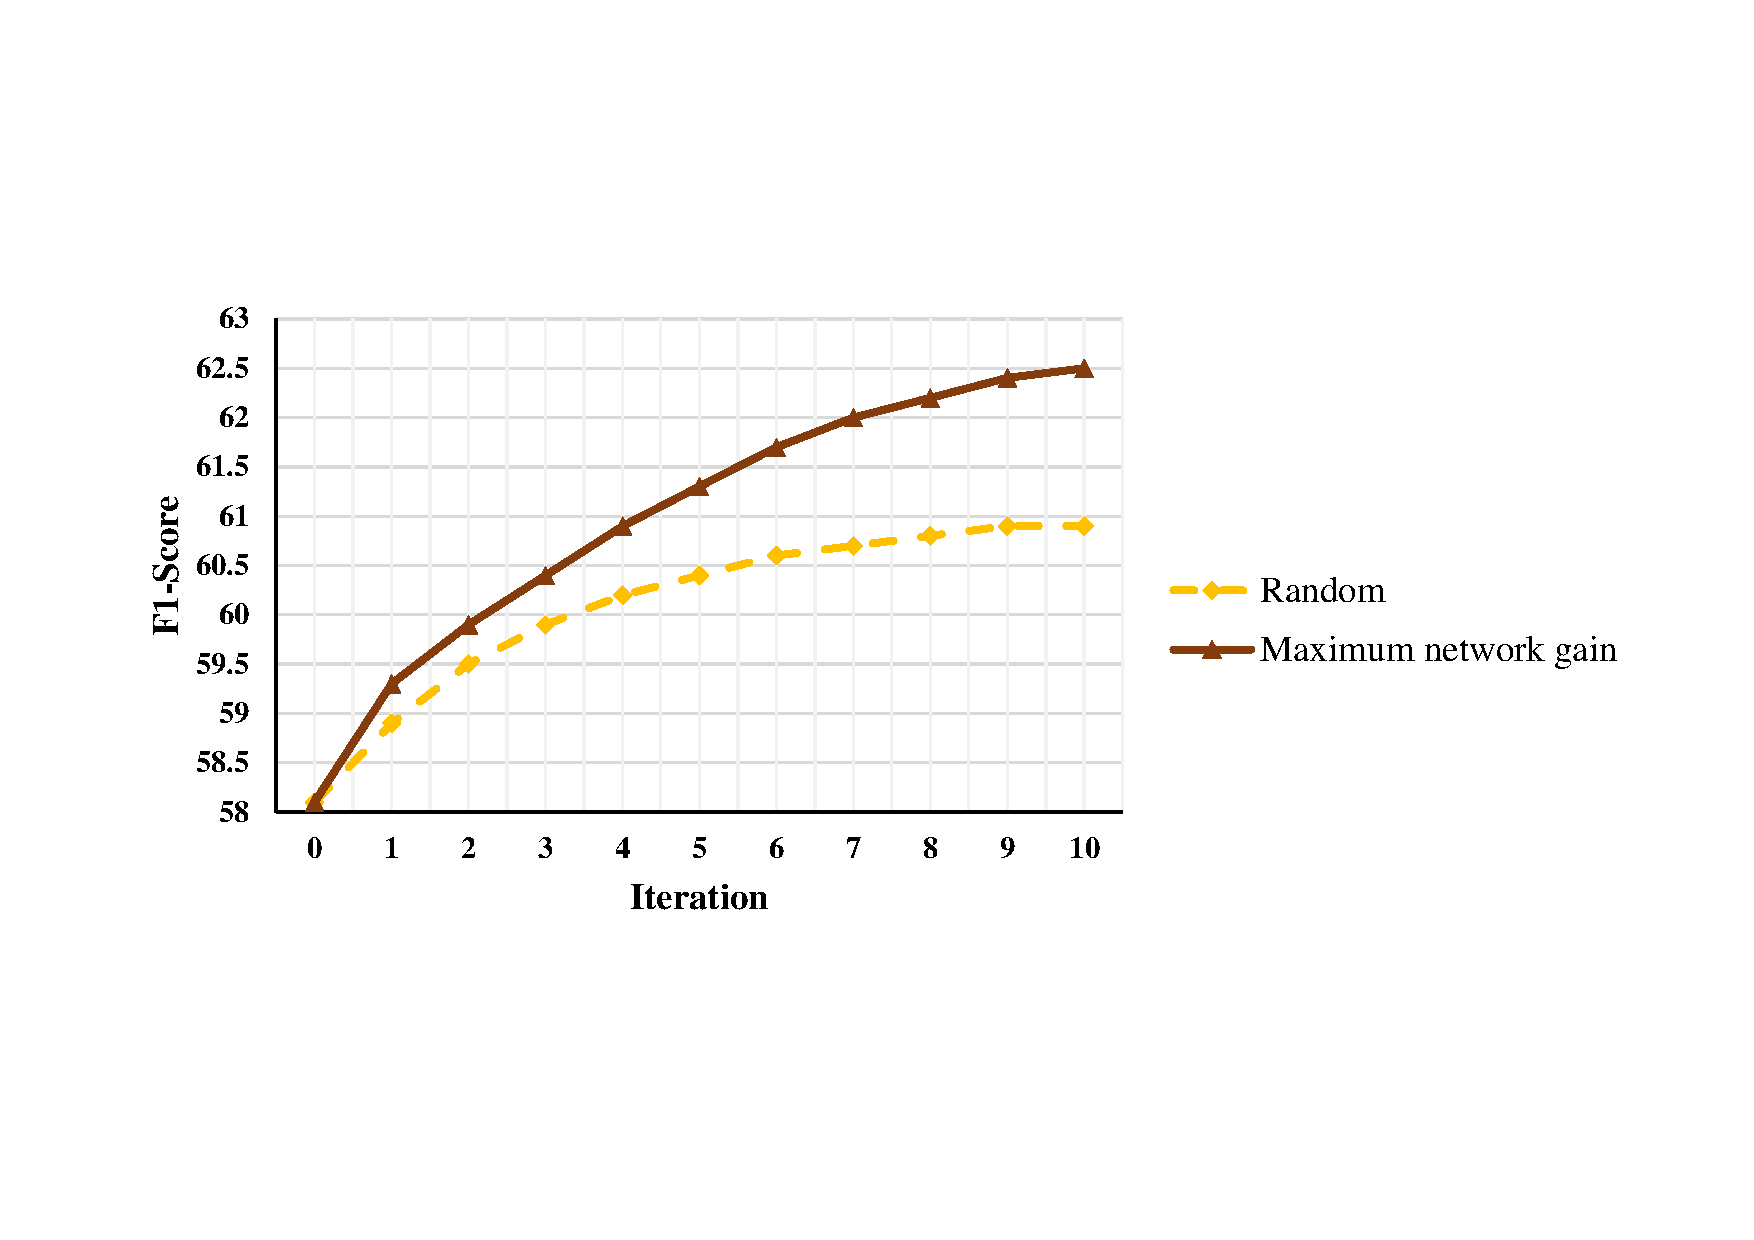
\includegraphics[width=5in]{img/chap3/AL_Comparison.pdf}
\caption{主动学习算法对预测的影响}
\label{fig_ResALComparison}
\end{figure*}

从图\ref{fig_ResALComparison}中可以看出,结合了最大批量网络增益采样策略主动学习算法的标签传播算法能够比随机采样有更好的表现。从第三次迭代开始,最大批量网络增益的主动学习算法与随机采样策略之间的差距逐渐变大,这样的趋势也表明本章提出的恶意软件检测系统的性能比其他的方法要好。

\section{本章小结}

\makeatletter
\addtocontents{lof}{\vspace{-10pt}}
\addtocontents{lot}{\vspace{-10pt}}
\makeatother

% \include{tex/zkc_chap4}

% \makeatletter
% \addtocontents{lof}{\vspace{-10pt}}
% \addtocontents{lot}{\vspace{-10pt}}
% \makeatother

% \include{tex/zkc_chap5}

% \makeatletter
% \addtocontents{lof}{\vspace{-10pt}}
% \addtocontents{lot}{\vspace{-10pt}}
% \makeatother

% \include{tex/zkc_chap6}
\chapter{总结与展望}


\backmatter
\ctexset{chapter/format={\bfseries\songti\zihao{3}}}
\begin{thanks}
%	值此论文完稿之际,
	
\end{thanks}
{\addcontentsline{toc}{chapter}{\bibname}\centering\bibliography{bib/thesis}}
\begin{appendix}

{\noindent\bf\songti\zihao{4}攻读博士学位期间发表的论文和出版著作情况:}

\begin{compactenum}[1.][17]
	\item 
	Kechen Zhuang, Haibo Shen, Hong Zhang: 
	User Spread Influence Measurement in Microblog. Multimedia Tools and Applications, 2016.
	(SCI在线发表, EI:20163202701002) 
	%\textbf{(第一作者)}
	
\end{compactenum}

\vspace{20pt}
{\noindent\bf\songti\zihao{4}攻读博士学位期间参加的科学研究情况:}

\begin{compactenum}[1.][17]
\item
Urban Population Activity Patterns Prediction based on Mobile Phone Data,华盛顿大学,南京理工大学出国访学资助,起止时间:2013年1月至2013年10月;
\end{compactenum}

\end{appendix}

\end{document}
